% !TEX program = tectonic
% Deck « La Chambre, de bout en bout » — la récupération House V1, propre et prouvée.
% Fil : site du Clerk → ZIP → index XML → les 12 FilingType (tableau) → périmètre (cycle de vie)
%      → lisible/scanné par préfixe DocID (prouvé) → paradoxe documents/transactions
%      → cohérence chronologique des portefeuilles (H + P ⊇ T, contrôlée par O/A).
% Tous les chiffres proviennent des tables versionnées 01_v1_house/cache/tables/*.csv et de
% cache/MANIFEST.json — vérifiés par asserts (scratchpad gen_figs_house.py) ; référence en
% commentaire sur chaque slide. Style identique à SLIDES_DONNEES_S1S2.tex.
\documentclass[11pt,aspectratio=169]{beamer}
\definecolor{helec}{HTML}{3B6EA5}   % couleur maîtresse (Chambre électronique)
\usetheme{Madrid}
\usecolortheme[named=helec]{structure}
\setbeamertemplate{navigation symbols}{}
\setbeamertemplate{blocks}[rounded][shadow=false]
\setbeamerfont{frametitle}{series=\bfseries}
\setbeamertemplate{section in toc}[sections numbered]
\setbeamerfont{section in toc}{size=\large}
\usepackage[T1]{fontenc}
\usepackage{lmodern}
\usepackage[utf8]{inputenc}
\usepackage[french]{babel}
\usepackage{booktabs}
\usepackage{xcolor}
\usepackage{graphicx}
\usepackage{fancyvrb}
\usepackage{amssymb}
\usepackage{textcomp}
\usepackage{array}
\usepackage{newunicodechar}
\usepackage{tikz}
\usetikzlibrary{arrows.meta,positioning,calc}
\graphicspath{{figs/}}   % AUTONOME : toutes les images vivent dans 01_v1_house/slides/figs/
\hypersetup{colorlinks=true, urlcolor=helec, linkcolor=white}

% Caractères Unicode → commandes (fontes T1)
\newunicodechar{→}{\ensuremath{\rightarrow}}
\newunicodechar{—}{\textemdash}
\newunicodechar{–}{\textendash}
\newunicodechar{…}{\ldots}
\newunicodechar{·}{\textperiodcentered}
\newunicodechar{≈}{\ensuremath{\approx}}
\newunicodechar{×}{\ensuremath{\times}}
\newunicodechar{≤}{\ensuremath{\leq}}
\newunicodechar{≥}{\ensuremath{\geq}}
\newunicodechar{−}{\ensuremath{-}}
\newunicodechar{✓}{\checkmark}
\newunicodechar{✗}{\ensuremath{\times}}
\newunicodechar{↔}{\ensuremath{\leftrightarrow}}
\newunicodechar{⊇}{\ensuremath{\supseteq}}
\newunicodechar{Σ}{\ensuremath{\Sigma}}
\newunicodechar{∧}{\ensuremath{\wedge}}
\newunicodechar{œ}{\oe}
\newunicodechar{Œ}{\OE}
\newunicodechar{°}{\textdegree}
\newunicodechar{§}{\S}
\newunicodechar{«}{\og}
\newunicodechar{»}{\fg{}}

% Code couleur (repris du deck S1S2 et des figures matplotlib)
\definecolor{helec}{HTML}{3B6EA5}   % Chambre électronique
\definecolor{hocr}{HTML}{A9C5E2}    % Chambre OCR
\definecolor{selec}{HTML}{8E44AD}   % Sénat électronique
\definecolor{socr}{HTML}{CFAEDE}    % Sénat OCR
\definecolor{okgreen}{HTML}{2E8B57}
\definecolor{alertred}{HTML}{C0392B}
\definecolor{warnorange}{HTML}{E67E22}
\definecolor{dataC}{RGB}{176,110,14}  % famille patrimoine (ocre)
\definecolor{grisC}{RGB}{90,90,90}    % cartes neutres (mixable en !10)

% Styles TikZ
\newcommand{\co}[1]{\texttt{#1}}
\tikzset{
  step/.style={rectangle, rounded corners=2pt, draw=#1, line width=0.8pt, fill=#1!8,
               align=center, font=\scriptsize, minimum height=0.72cm},
  bande/.style={rectangle, rounded corners=2pt, draw=#1, line width=0.8pt, fill=#1!8,
                align=center, font=\scriptsize, minimum height=0.62cm},
  arr/.style={-{Latex[length=2mm]}, line width=0.8pt, draw=gray!65},
}

% Tuile chiffre-clé : \tuile{couleur}{gros chiffre}{légende}
\newcommand{\tuile}[3]{%
  \begin{minipage}[t]{0.23\textwidth}\centering
    \colorbox{#1}{\parbox[c][21mm][c]{\dimexpr\linewidth-8pt}{\centering
      {\color{white}\Large\textbf{#2}}\\[0.6mm]
      {\color{white}\footnotesize #3}}}
  \end{minipage}}

% Badge coloré une ligne
\newcommand{\badge}[2]{\colorbox{#1}{\textcolor{white}{\footnotesize\textbf{#2}}}}
\newcommand{\badgel}[2]{\colorbox{#1}{\textcolor{black!80}{\footnotesize\textbf{#2}}}}

\title[La Chambre, de bout en bout]{La Chambre, de bout en bout}
\subtitle{Du site du Clerk au portefeuille de chaque élu — la récupération V1, propre et prouvée}
\author[A.~Lemaire]{Alice Lemaire}
\institute[Ramify]{Document de recherche — livrable Ramify}
\date{Juillet 2026}

\begin{document}

\section{La source — le site du Clerk, un ZIP, un index XML}

% ── H1 · Page de titre ──
\begin{frame}[plain]
  \titlepage
\end{frame}

% ── H2 · Le fil ── (7 actes chronologiques ; sommaire manuel — la TOC hyperref serait blanche)
\begin{frame}{Le fil — sept actes, dans l'ordre du réel}
  \centering
  \colorbox{helec}{\parbox{0.9\textwidth}{\scriptsize\color{white}
    \textbf{1 · La source} — le site du Clerk, un ZIP par année, un index XML par dépôt}}\\[1.5mm]
  \colorbox{dataC}{\parbox{0.9\textwidth}{\scriptsize\color{white}
    \textbf{2 · L'inventaire} — les 12 FilingType et les sections A→J du formulaire}}\\[1.5mm]
  \colorbox{okgreen}{\parbox{0.9\textwidth}{\scriptsize\color{white}
    \textbf{3 · La chronologie d'un élu} — candidature C → entrée H → mandat P/O/A → sortie T}}\\[1.5mm]
  \colorbox{hocr}{\parbox{0.9\textwidth}{\scriptsize\color{black!80}
    \textbf{4 · Les documents} — lisible ou scanné, le préfixe du DocID le dit (et on l'a prouvé)}}\\[1.5mm]
  \colorbox{grisC}{\parbox{0.9\textwidth}{\scriptsize\color{white}
    \textbf{5 · Rien d'oublié} — 35\,377 dépôts, un traitement chacun, la somme boucle}}\\[1.5mm]
  \colorbox{warnorange}{\parbox{0.9\textwidth}{\scriptsize\color{white}
    \textbf{6 · Les portefeuilles} — entrée + transactions ⊇ sortie, membre par membre}}\\[1.5mm]
  \colorbox{alertred}{\parbox{0.9\textwidth}{\scriptsize\color{white}
    \textbf{7 · Verdict} — ce qui est prouvé, ce qui reste}}\\[3mm]
  {\scriptsize\color{black!55} tous les chiffres sortent des tables versionnées
   (\co{01\_v1\_house/cache/tables/} + \co{MANIFEST.json}) — 57 validations, 0 rouge}
\end{frame}

% ── H3 · Le site du Clerk + la purge ── (recensement : 01_recensement_depots.csv, union site∪instantané)
\begin{frame}{La source (1/2) — le site officiel : une archive par année}
  \begin{columns}[T]
    \begin{column}{0.60\textwidth}\centering
      \fcolorbox{black!25}{white}{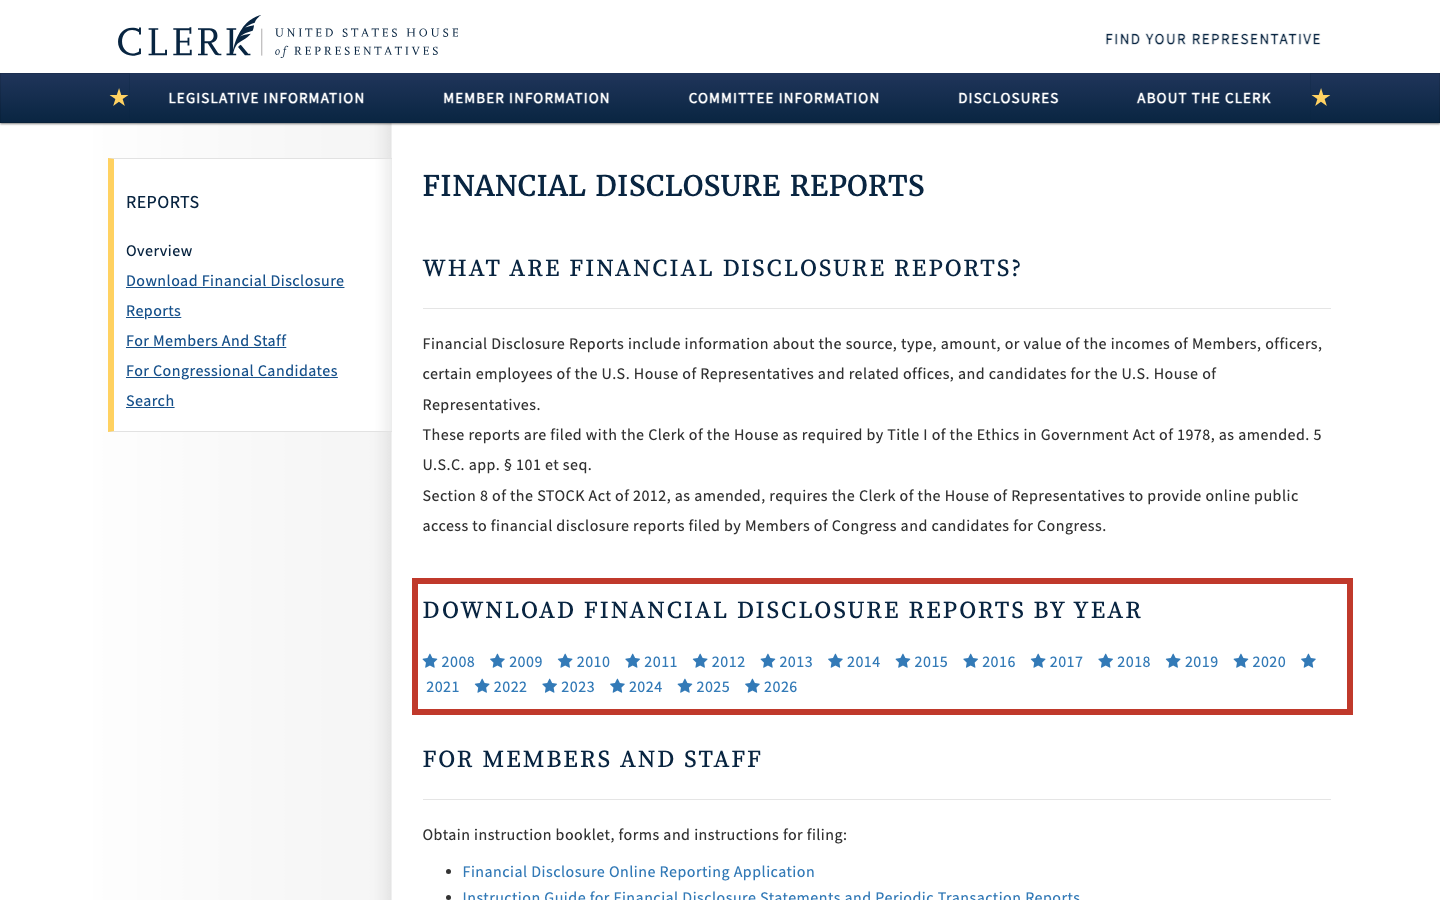
\includegraphics[width=0.97\linewidth]{slides/site_house_clerk.png}}\\[0.8mm]
      {\footnotesize \href{https://disclosures-clerk.house.gov/FinancialDisclosure}%
       {\texttt{disclosures-clerk.house.gov}}} {\scriptsize\color{black!55}(cliquable)}
    \end{column}
    \begin{column}{0.38\textwidth}
      {\footnotesize la récupération V1 repart de zéro :}\\[1.5mm]
      {\footnotesize
      · une \textbf{archive ZIP par année}, \co{2014FD.zip} → \co{2026FD.zip}\\[1.2mm]
      · re-téléchargées \textbf{toutes}, juillet 2026}\\[2.5mm]
      \colorbox{alertred!10}{\parbox{0.96\linewidth}{\scriptsize
        \textbf{\textcolor{alertred}{la source s'efface — et c'est la loi}} :
        \href{https://www.law.cornell.edu/uscode/text/5/13107}{5 U.S.C. §13107(d)}
        impose la \textbf{destruction} — 6 ans après le dépôt (candidats, employés),
        6 ans après la \textbf{fin du mandat} (élus). Le Clerk purge l'index
        \textbf{par année entière, en retard} : \textbf{2014 = 99,6 \% effacé}
        (2\,784 dépôts ne survivent que chez nous) ; 2015→2026 intacts
        (re-vérifié le 13/07/2026). Seule la \emph{liste} meurt — les PDF restent
        servis… pour l'instant.}}\\[2mm]
      \badge{helec}{35\,377 dépôts recensés · 2014-2026}
    \end{column}
  \end{columns}
\end{frame}

% ── H4 · ZIP → index XML : les champs ── (9 champs par <Member> ; V1_House.ipynb §1)
\begin{frame}{La source (2/2) — dans le ZIP, l'index XML : un bloc par dépôt}
  \begin{columns}[T]
    \begin{column}{0.42\textwidth}
      \centering
      \begin{tikzpicture}[node distance=5mm]
        \node[step=helec, text width=4.5cm] (z) {l'archive de l'année\\[1mm]\co{2024FD.zip}};
        \node[step=helec, text width=4.5cm, below=of z] (x) {dézippée → un fichier\\[1mm]\co{2024FD.xml}};
        \node[step=grisC, text width=4.5cm, below=of x] (i) {l'\textbf{index annuel} :\\un bloc \co{<Member>} par \textbf{dépôt}};
        \draw[arr] (z) -- (x); \draw[arr] (x) -- (i);
      \end{tikzpicture}\\[1.5mm]
      {\scriptsize\color{black!55} \href{https://disclosures-clerk.house.gov/public_disc/financial-pdfs/2024FD.zip}%
       {\texttt{…/financial-pdfs/2024FD.zip}}}
    \end{column}
    \begin{column}{0.56\textwidth}\centering
      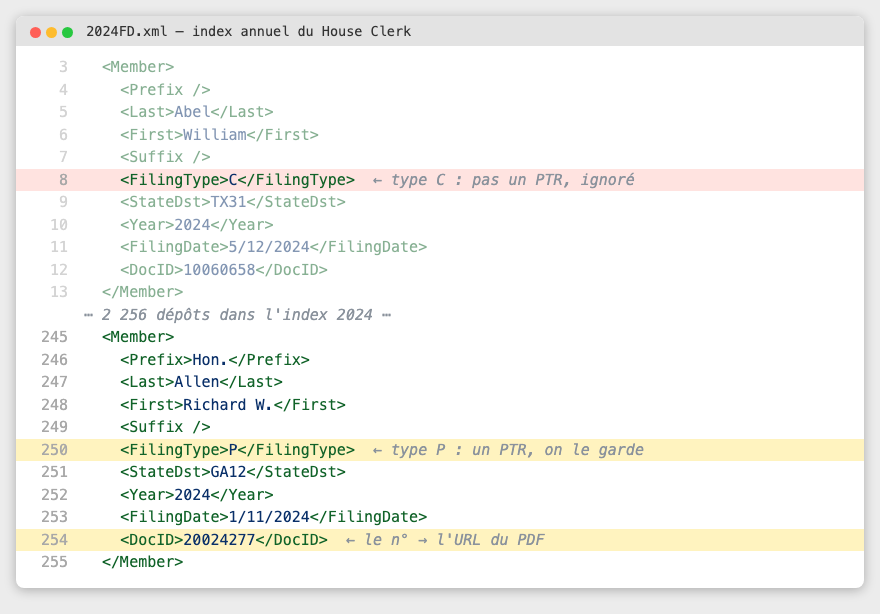
\includegraphics[width=0.92\linewidth]{slides/fichier_index_xml.png}\\[1.5mm]
      \colorbox{grisC!10}{\parbox{0.97\linewidth}{\scriptsize
        \textbf{9 champs par dépôt} : \co{Prefix} · \co{Last} · \co{First} · \co{Suffix} ·
        \co{StateDst} · \co{Year} · \co{FilingDate} ·
        {\color{helec}\textbf{\co{FilingType}}} — \emph{quel genre de dépôt ?} ·
        {\color{helec}\textbf{\co{DocID}}} — \emph{la clé qui ouvre le PDF, et qui dit
        s'il sera lisible}}}
    \end{column}
  \end{columns}
\end{frame}

\section{L'inventaire — 12 FilingType, et les sections A→J du formulaire}

% ── H5 · LA TABLE FilingType × année ── (source : 01_recensement_depots.csv, 35 377 ; asserts gen_figs_house.py)
\begin{frame}{Les 12 \texttt{FilingType} — tout l'index, compté type par type}
  \centering
  {\setlength{\tabcolsep}{3pt}\scriptsize
  \begin{tabular}{l rrrrrrrrrrrrr r r}
    \toprule
    & 2014 & 2015 & 2016 & 2017 & 2018 & 2019 & 2020 & 2021 & 2022 & 2023 & 2024 & 2025 & 2026 & total & \% \\
    \midrule
    \textcolor{dataC}{\textbf{C}} & 776 & 401 & 715 & 1\,001 & 1\,075 & 964 & 780 & 753 & 861 & 621 & 661 & 892 & 629 & \textbf{10\,129} & 28,6\,\% \\
    \textcolor{helec}{\textbf{P}} & 708 & 728 & 765 & 801 & 830 & 683 & 733 & 680 & 624 & 460 & 451 & 515 & 289 & \textbf{8\,267} & 23,4\,\% \\
    \textcolor{black!45}{X} & 208 & 298 & 299 & 509 & 319 & 743 & 567 & 489 & 464 & 553 & 454 & 709 & 239 & \textbf{5\,851} & 16,5\,\% \\
    \textcolor{dataC}{\textbf{O}} & 397 & 440 & 393 & 437 & 355 & 434 & 374 & 432 & 367 & 431 & 372 & 194 & · & \textbf{4\,626} & 13,1\,\% \\
    \textcolor{dataC}{\textbf{A}} & 310 & 213 & 230 & 256 & 239 & 202 & 161 & 164 & 180 & 129 & 103 & 89 & 29 & \textbf{2\,305} & 6,5\,\% \\
    \textcolor{black!45}{D} & 224 & 130 & 164 & 336 & 228 & 413 & 164 & 116 & 86 & 79 & 70 & 132 & 57 & \textbf{2\,199} & 6,2\,\% \\
    \textcolor{black!45}{W} & 109 & 31 & 87 & 91 & 279 & 107 & 83 & 19 & 71 & 19 & 66 & 47 & 93 & \textbf{1\,102} & 3,1\,\% \\
    \textcolor{dataC}{\textbf{H}} & 50 & · & 45 & · & 87 & · & 62 & 1 & 76 & 4 & 66 & 2 & 2 & \textbf{395} & 1,1\,\% \\
    \textcolor{dataC}{\textbf{T}} & 7 & 50 & 5 & 49 & 6 & 85 & 4 & 53 & 8 & 65 & 7 & 53 & 2 & \textbf{394} & 1,1\,\% \\
    \textcolor{black!45}{G} & 5 & 1 & 1 & 1 & 22 & · & · & 4 & 1 & 8 & 3 & 5 & · & \textbf{51} & 0,1\,\% \\
    \textcolor{black!45}{E} & 1 & 5 & · & 7 & 2 & 5 & 2 & 4 & · & 3 & 1 & 5 & · & \textbf{35} & 0,1\,\% \\
    \textcolor{black!45}{B} & · & · & · & · & 1 & · & · & 3 & 6 & 7 & 4 & 2 & · & \textbf{23} & 0,1\,\% \\
    \midrule
    total & 2\,795 & 2\,297 & 2\,704 & 3\,488 & 3\,443 & 3\,636 & 2\,930 & 2\,718 & 2\,744 & 2\,379 & 2\,258 & 2\,645 & 1\,340 & \textbf{35\,377} & 100\,\% \\
    \bottomrule
  \end{tabular}}\\[1.8mm]
  {\footnotesize \badge{helec}{P = le signal}\;
   \badgel{dataC!30}{\textcolor{dataC}{\textbf{O·C·H·T·A} = le patrimoine}}\;
   {\color{black!50}\textbf{X·D·W·G·E·B} = administratif ou à part}}\\[0.8mm]
  {\scriptsize\color{black!55} unité : dépôt · recensement V1 = union site $\cup$
   instantané (les creux des H suivent le calendrier électoral)}
\end{frame}

% ── H6 · Famille patrimoine (reprise deck S1S2, comptes V1) ── (recensement V1)
\begin{frame}{À quoi correspond chaque type (1/2) — la famille « patrimoine »}
  \centering
  {\footnotesize cinq types, un socle commun (le \emph{Financial Disclosure Report}) —
   les \textbf{transactions (Schedule B) n'existent que dans O, T et leurs amendements}}\\[2mm]
  \begin{columns}[T]
    \begin{column}{0.19\textwidth}\centering
      \href{https://disclosures-clerk.house.gov/public_disc/financial-pdfs/2023/10059952.pdf}{\fcolorbox{black!30}{white}{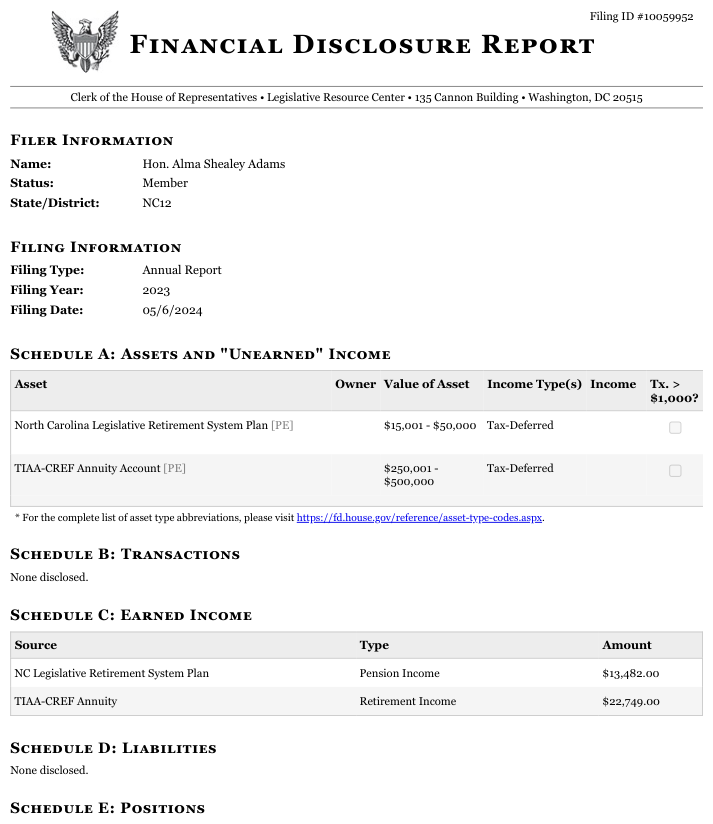
\includegraphics[height=29mm]{slides/ftype_o.png}}}\\[0.8mm]
      {\footnotesize\textbf{O — Annual}}\\{\scriptsize bilan annuel · \textbf{4\,626}}
\end{column}
    \begin{column}{0.19\textwidth}\centering
      \href{https://disclosures-clerk.house.gov/public_disc/financial-pdfs/2023/10056211.pdf}{\fcolorbox{black!30}{white}{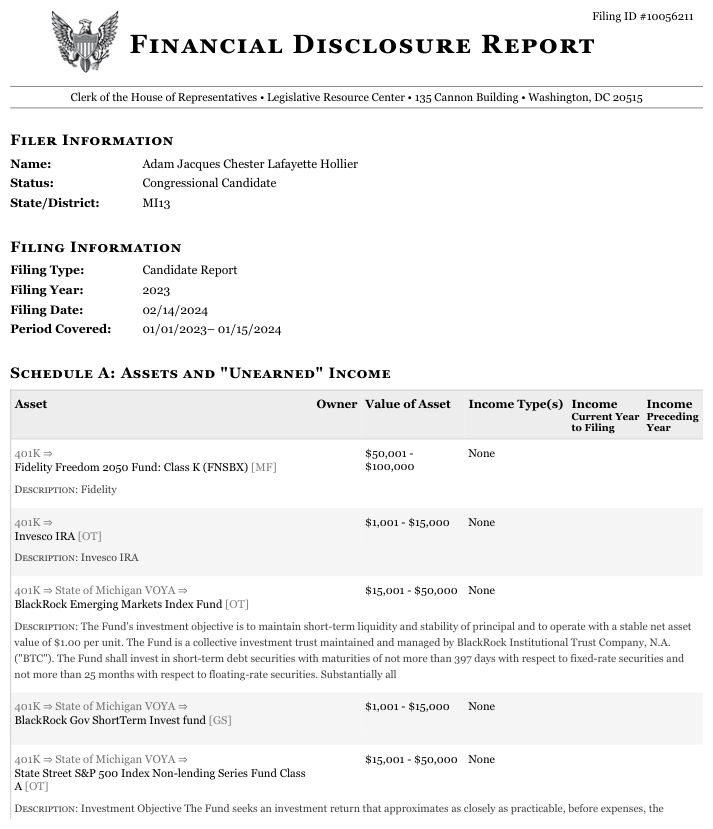
\includegraphics[height=29mm]{slides/ftype_c.png}}}\\[0.8mm]
      {\footnotesize\textbf{C — Candidate}}\\{\scriptsize candidat · \textbf{10\,129}}
\end{column}
    \begin{column}{0.19\textwidth}\centering
      \href{https://disclosures-clerk.house.gov/public_disc/financial-pdfs/2023/10062638.pdf}{\fcolorbox{black!30}{white}{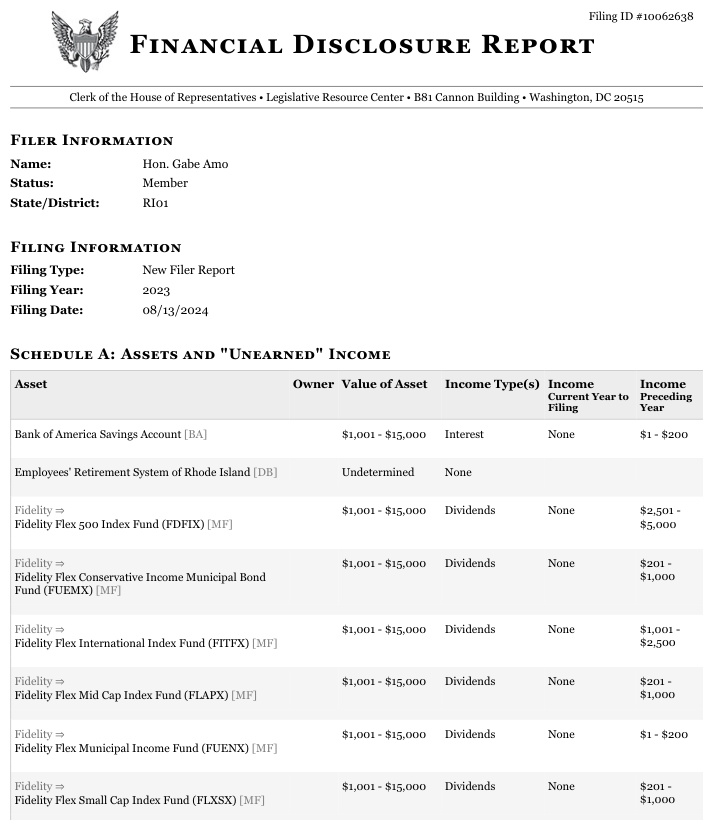
\includegraphics[height=29mm]{slides/ftype_h.png}}}\\[0.8mm]
      {\footnotesize\textbf{H — New Filer}}\\{\scriptsize 1\iere{} déclaration · \textbf{395}}
\end{column}
    \begin{column}{0.19\textwidth}\centering
      \href{https://disclosures-clerk.house.gov/public_disc/financial-pdfs/2023/10050798.pdf}{\fcolorbox{black!30}{white}{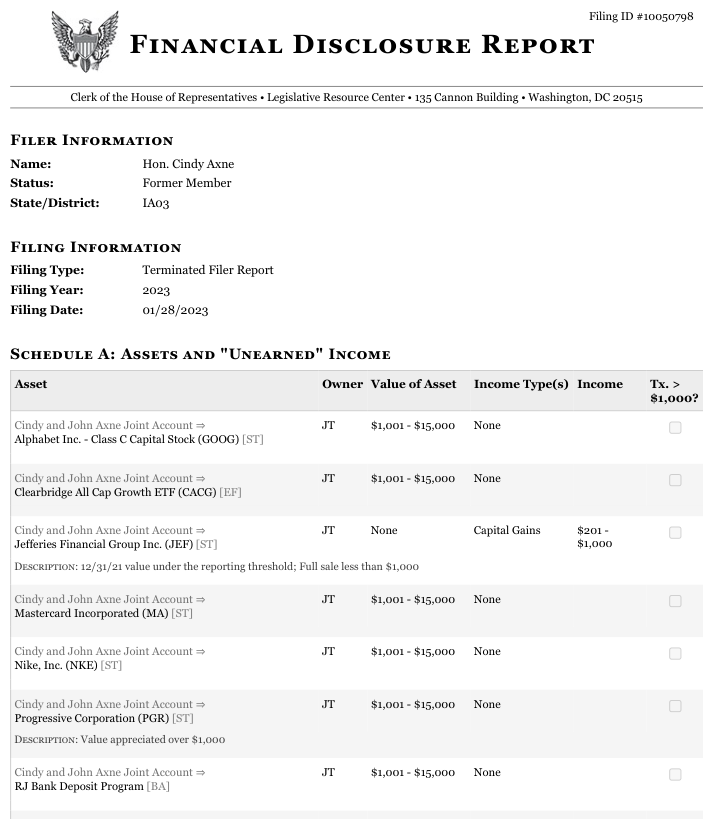
\includegraphics[height=29mm]{slides/ftype_t.png}}}\\[0.8mm]
      {\footnotesize\textbf{T — Termination}}\\{\scriptsize départ · \textbf{394}}
\end{column}
    \begin{column}{0.19\textwidth}\centering
      \href{https://disclosures-clerk.house.gov/public_disc/financial-pdfs/2023/10062190.pdf}{\fcolorbox{black!30}{white}{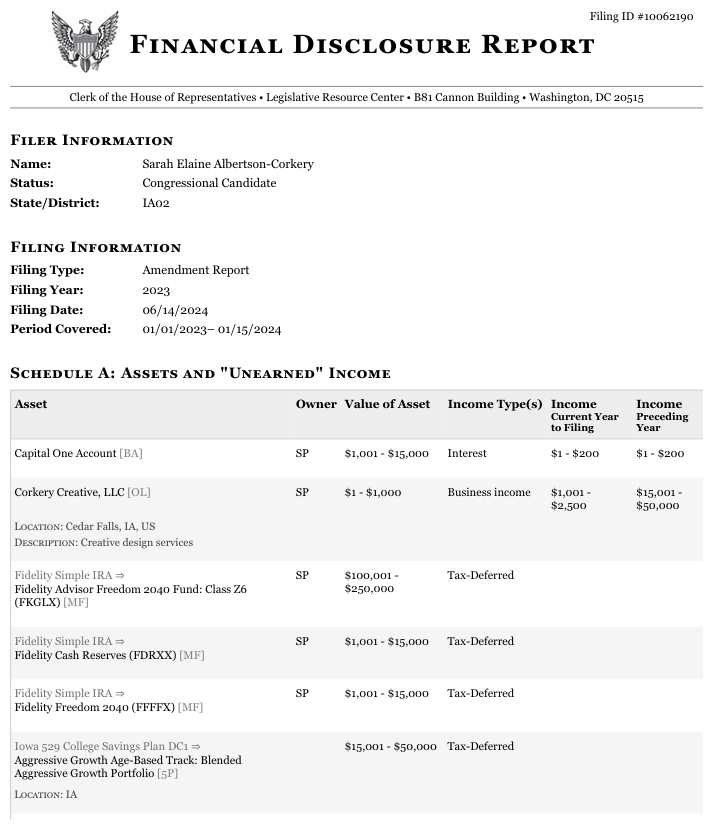
\includegraphics[height=29mm]{slides/ftype_a.png}}}\\[0.8mm]
      {\footnotesize\textbf{A — Amendment}}\\{\scriptsize correction · \textbf{2\,305}}
\end{column}
  \end{columns}
  \vspace{2.5mm}
  \badge{helec}{chaque vignette est cliquable → ouvre le vrai document}\quad
  {\scriptsize\color{black!60} significations vérifiées en ouvrant les documents ·
   détail par type : acte 3}
\end{frame}

% ── H6a · Les sections A→J (matrice) ── (fig_sections_matrix, repris S1S2 — structure du formulaire)
\begin{frame}{Le formulaire de l'intérieur — des sections A→J en commun}
  \centering
  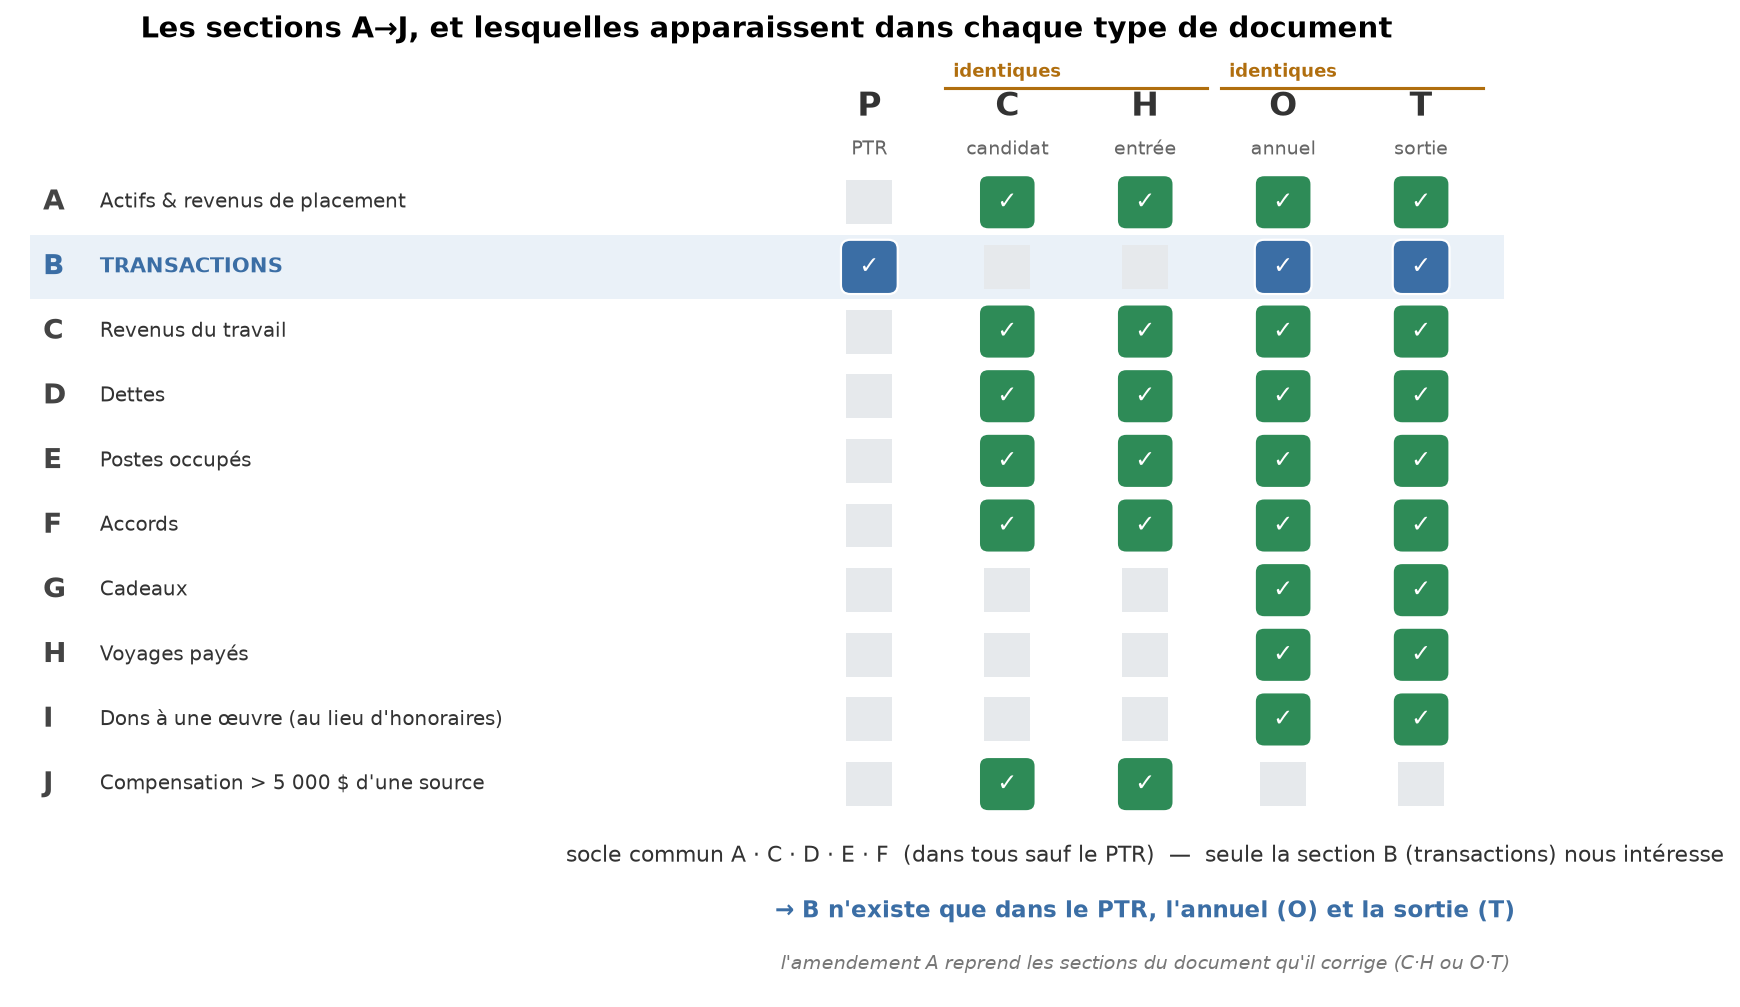
\includegraphics[width=0.72\textwidth]{slides/fig_sections_matrix.png}\\[1mm]
  {\scriptsize\color{black!60} tous ces documents partagent un socle (A·C·D·E·F) —
   ce qui change d'un type à l'autre, c'est surtout la présence de la
   \textbf{section B, les transactions}}
\end{frame}

% ── H6b · Le rôle des sections ── (fig_sections_roles, repris S1S2)
\begin{frame}{Les sections A→J — laquelle est le signal ?}
  \centering
  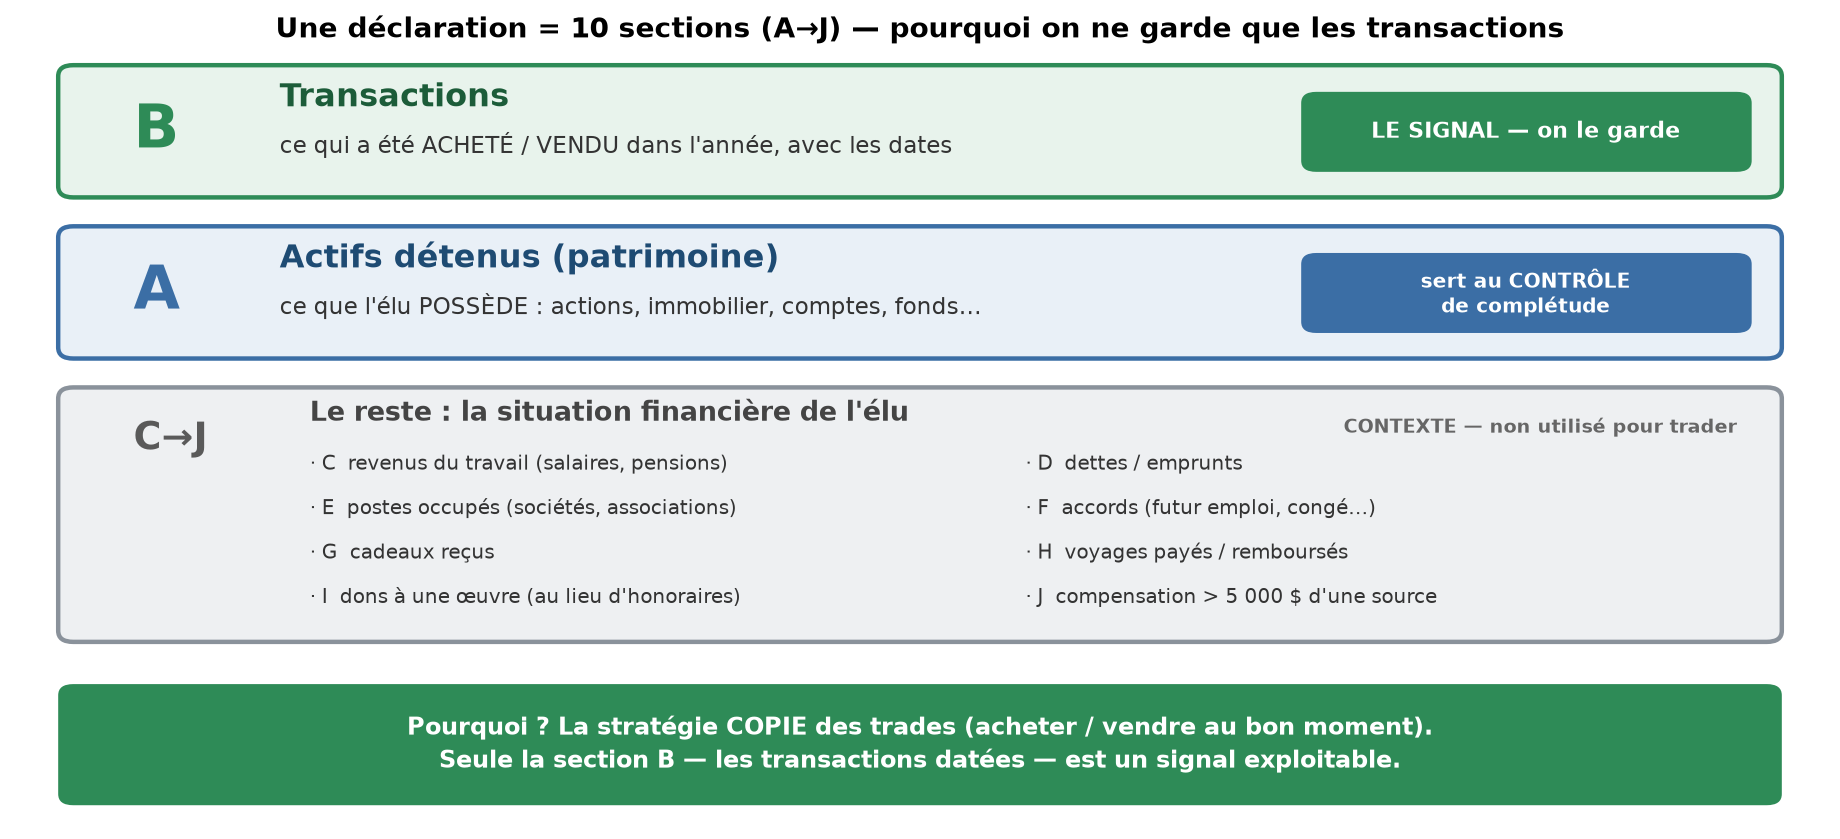
\includegraphics[width=0.88\textwidth]{slides/fig_sections_roles.png}\\[1mm]
  {\footnotesize on trade la \textbf{section B} (transactions datées) ; la
   \textbf{section A} (patrimoine) sert seulement à \emph{vérifier} qu'on n'a rien
   loupé — c'est tout l'objet de l'acte 6}
\end{frame}

% ── H7 · Administratifs + blind trust (reprise deck S1S2, comptes V1) ──
\begin{frame}{À quoi correspond chaque type (2/2) — les administratifs, et le cas à part}
  \centering
  {\footnotesize cinq types \textbf{sans aucune transaction} :}\\[1.5mm]
  \begin{columns}[T]
    \begin{column}{0.19\textwidth}\centering
      \fcolorbox{black!30}{white}{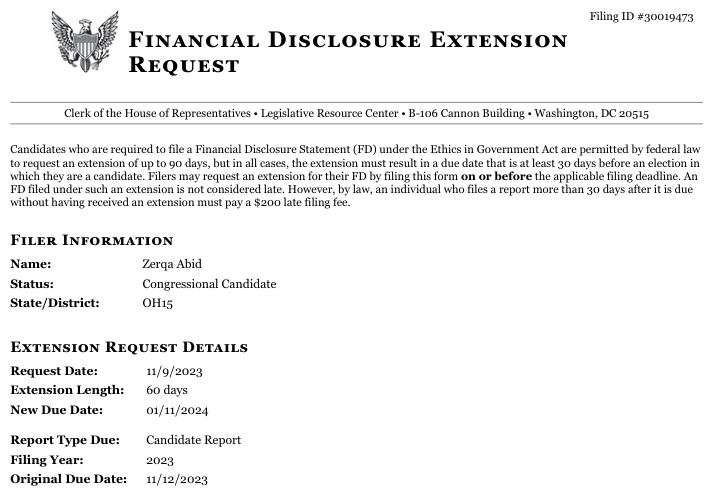
\includegraphics[height=20mm]{slides/ftype_x.png}}\\[0.6mm]
      {\scriptsize\textbf{X — Extension}\\délai · \textbf{5\,851}}
    \end{column}
    \begin{column}{0.19\textwidth}\centering
      \fcolorbox{black!30}{white}{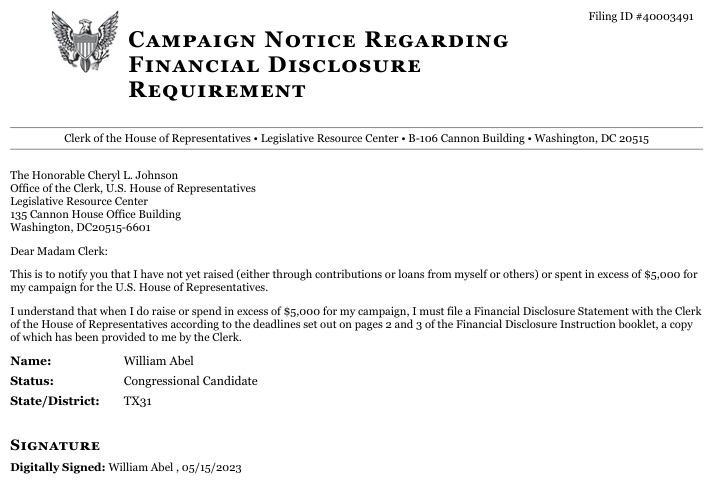
\includegraphics[height=20mm]{slides/ftype_d.png}}\\[0.6mm]
      {\scriptsize\textbf{D — Camp. Notice}\\\textless\,5\,000 \$ levés · \textbf{2\,199}}
    \end{column}
    \begin{column}{0.19\textwidth}\centering
      \fcolorbox{black!30}{white}{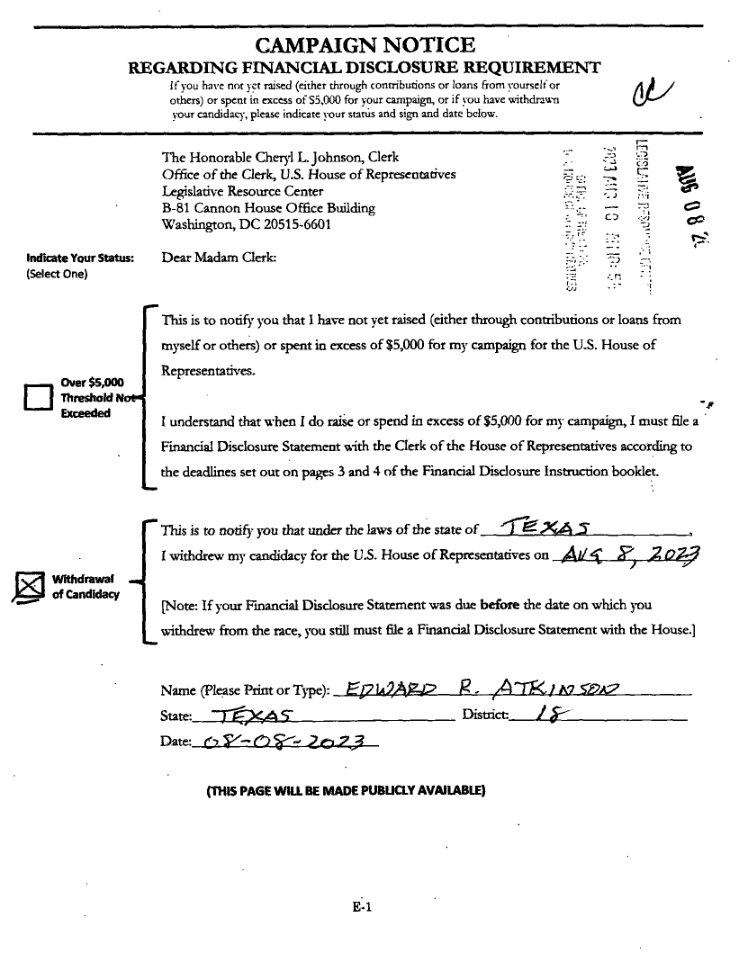
\includegraphics[height=20mm]{slides/ftype_w.png}}\\[0.6mm]
      {\scriptsize\textbf{W — idem, papier}\\(ou retrait) · \textbf{1\,102}}
    \end{column}
    \begin{column}{0.19\textwidth}\centering
      \fcolorbox{black!30}{white}{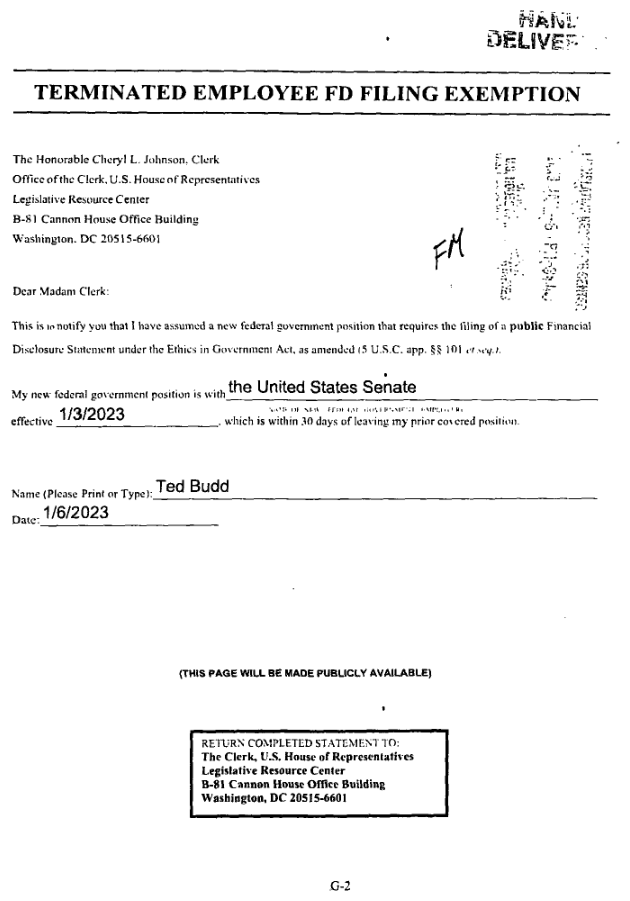
\includegraphics[height=20mm]{slides/ftype_e.png}}\\[0.6mm]
      {\scriptsize\textbf{E — Exemption}\\poste fédéral · \textbf{35}}
    \end{column}
    \begin{column}{0.19\textwidth}\centering
      \fcolorbox{black!30}{white}{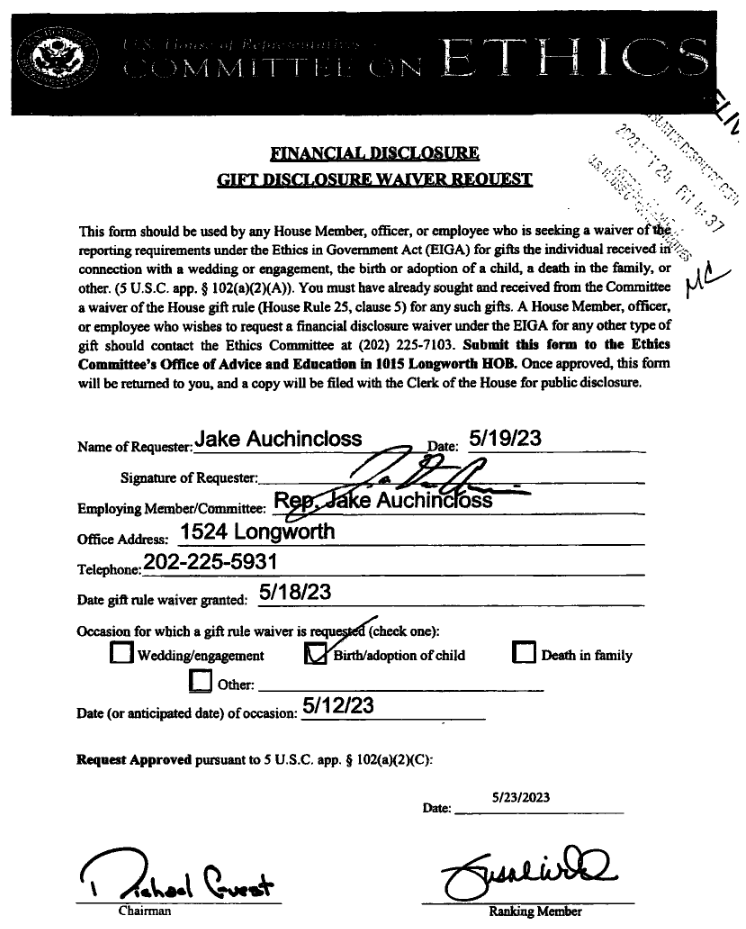
\includegraphics[height=20mm]{slides/ftype_g.png}}\\[0.6mm]
      {\scriptsize\textbf{G — Gift Waiver}\\dérogation cadeau · \textbf{51}}
    \end{column}
  \end{columns}
  \vspace{2.5mm}
  \begin{columns}[c]
    \begin{column}{0.14\textwidth}\centering
      \fcolorbox{alertred}{white}{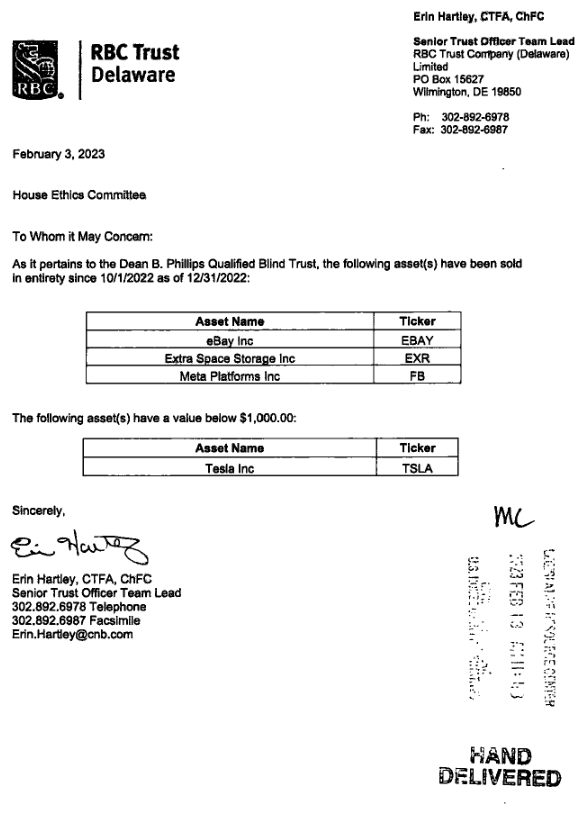
\includegraphics[height=19mm]{slides/ftype_b.png}}
    \end{column}
    \begin{column}{0.80\textwidth}
      \colorbox{alertred!10}{\parbox{0.97\linewidth}{\footnotesize
        \textbf{\textcolor{alertred}{B — Blind Trust}} (23 dépôts) : la banque du
        \emph{trust} liste des ventes (eBay, Meta, Tesla…) — de vraies transactions,
        mais \textbf{pas décidées par l'élu} : c'est le principe de la fiducie aveugle.}}
    \end{column}
  \end{columns}
\end{frame}

\section{La chronologie d'un élu — de la candidature à la sortie}

% ── H8 · Le cycle de vie = le périmètre ── (fig_cycle_vie ; périmètre V1 : P + O/C/H/T/A)
\begin{frame}{Ceux qu'on garde — le cycle de vie d'un élu dicte le périmètre}
  \centering
  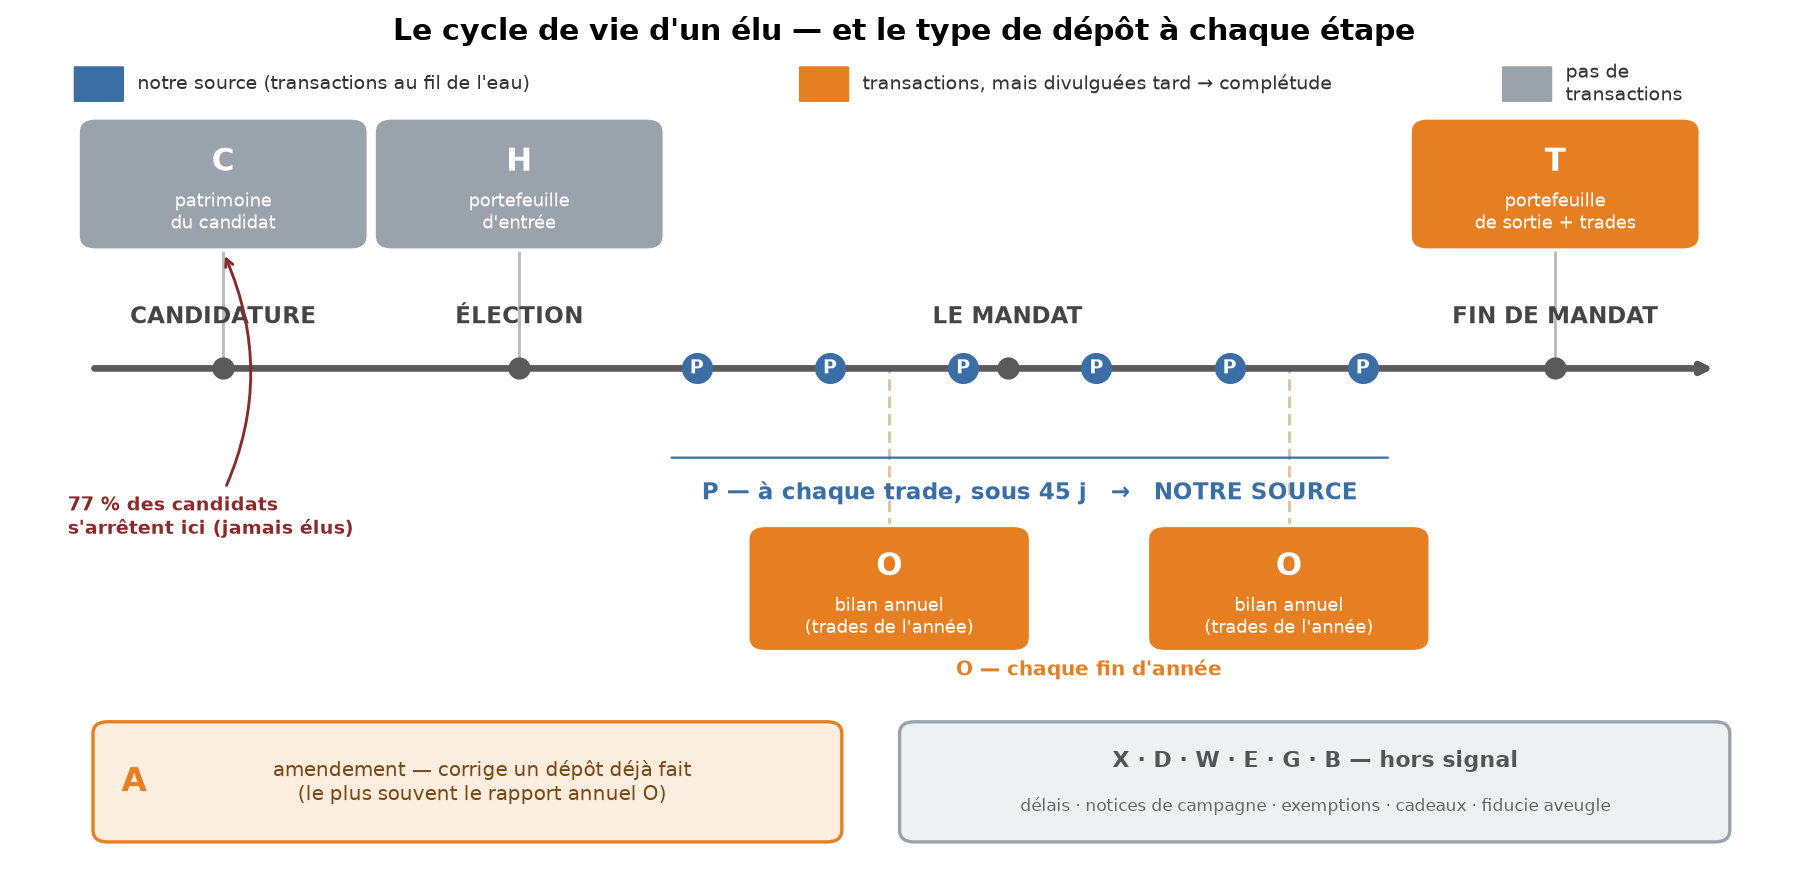
\includegraphics[width=0.70\textwidth]{slides/fig_cycle_vie.png}\\[1mm]
  \begin{columns}[T]
    \begin{column}{0.32\textwidth}\centering
      \colorbox{helec}{\parbox{0.96\linewidth}{\footnotesize\color{white}\centering
        \textbf{P — au fil de l'eau}\\le SIGNAL : daté au trade,\\divulgué $\approx$ 28 j après}}
    \end{column}
    \begin{column}{0.32\textwidth}\centering
      \colorbox{dataC}{\parbox{0.96\linewidth}{\footnotesize\color{white}\centering
        \textbf{C·H → O·A → T}\\le PATRIMOINE : photo d'entrée,\\bilans annuels, photo de sortie}}
    \end{column}
    \begin{column}{0.32\textwidth}\centering
      \colorbox{grisC}{\parbox{0.96\linewidth}{\footnotesize\color{white}\centering
        \textbf{X·D·W·G·E·B}\\administratif ou fiducie :\\rien à extraire pour le signal}}
    \end{column}
  \end{columns}
  \vspace{1.5mm}
  {\scriptsize\color{black!60} le patrimoine ne sert pas à trader (divulgation médiane
   \textbf{371 j}) — il sert à \textbf{vérifier} le flux P : c'est l'acte 6}
\end{frame}

% ── H8a · La loi du parcours, en un schéma ── (workflow source-primaire vérifié :
%    5 U.S.C. §13103 dépôts, §13105 STOCK Act PTR, §13103(e) exemption de sortie)
\begin{frame}{Comment on entre au Congrès : qui dépose quoi, et quand (la loi)}
  \centering
  
\includegraphics[width=0.72\textwidth]{fig_house_loi_cycle.png}\\[1mm]
  {\footnotesize \badge{alertred}{2 dérogations de la loi}\;
   un candidat déjà déclaré \textbf{saute le H} (§13103) ;
   qui rejoint le Sénat ou l'exécutif \textbf{ne dépose pas de T} (§13103(e))}\\[1.2mm]
  {\footnotesize
   \badge{okgreen}{ENTRÉES}\; sur \textbf{470} : \textbf{82,1 \%} un H, \textbf{98,1 \%} un H \emph{ou} un C\quad
   \badge{dataC}{SORTIES}\; sur \textbf{463} : \textbf{81,4 \%} un T}\\[0.8mm]
  {\scriptsize\color{black!55} le reste des T manquants = décès / départs très récents
   (cas de fait) · mesuré au §15 du notebook (validations D-1, D-2)}
\end{frame}

% ── AN2 · C ── (recensement V1 : 10 129 ; ledger : 8 533/1 583)
\begin{frame}{La candidature — \texttt{C}, le rapport du candidat}
  \begin{columns}[c]
    \begin{column}{0.34\textwidth}\centering
      \href{https://disclosures-clerk.house.gov/public_disc/financial-pdfs/2023/10056211.pdf}{\fcolorbox{black!30}{white}{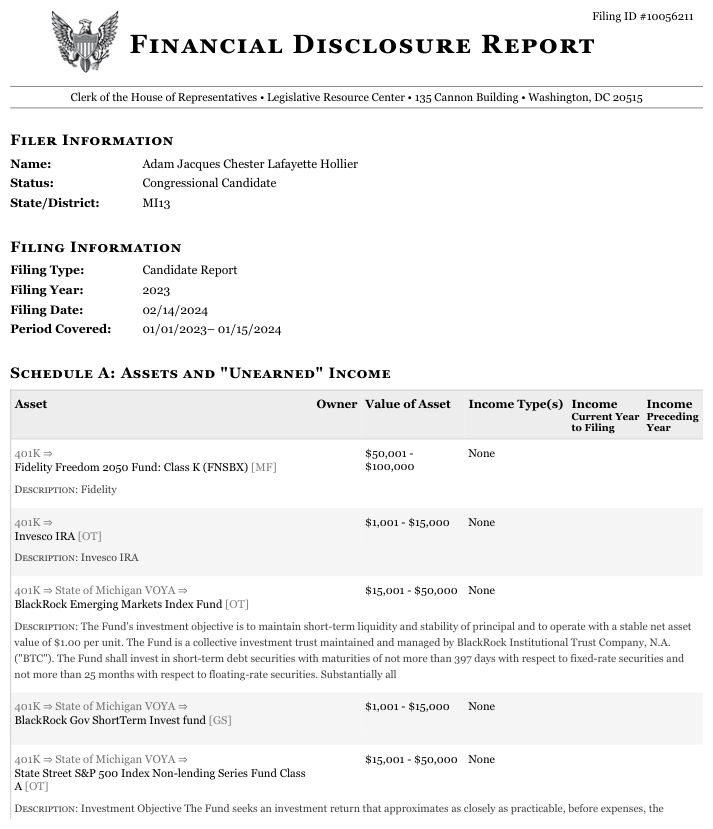
\includegraphics[height=54mm]{slides/ftype_c.png}}}\\[0.5mm]
      {\scriptsize\color{black!60} Adam Hollier, candidat MI13, 2023 — cliquable}
    \end{column}
    \begin{column}{0.64\textwidth}
      {\footnotesize
      \textbf{Qui, quand} — toute personne qui \textbf{se porte candidate} à la
      Chambre (une fois sa campagne au-delà de 5\,000 \$) — avant d'être élue, et
      le plus souvent sans jamais l'être.\\[1.2mm]
      \textbf{Ce qu'il contient} — la photo du patrimoine du candidat :
      actifs (A), salaires (C), dettes (D), postes (E), accords (F),
      compensations >\,5\,000 \$ (J). \textbf{Pas de section transactions} —
      0 sur les 39 échantillonnés.\\[1.2mm]
      \textbf{En chiffres} — \textbf{10\,129} dépôts, le type le plus fréquent de
      l'index · \textbf{77 \% déposés par des candidats jamais élus} ·
      3 pages en médiane.}\\[1.5mm]
      \badgel{grisC!30}{sans transactions — mais photo d'entrée de ceux qui seront élus}
    \end{column}
  \end{columns}
\end{frame}

% ── AN3 · H ── (recensement V1 : 395 ; ledger : 383/12)
\begin{frame}{L'entrée en fonction — \texttt{H}, la photo de départ du portefeuille}
  \begin{columns}[c]
    \begin{column}{0.34\textwidth}\centering
      \href{https://disclosures-clerk.house.gov/public_disc/financial-pdfs/2023/10062638.pdf}{\fcolorbox{black!30}{white}{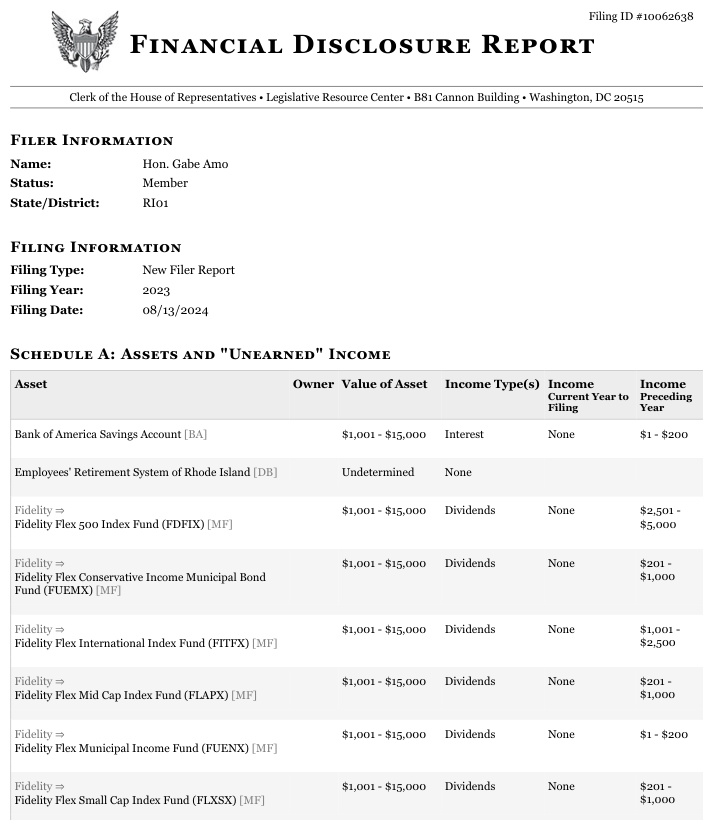
\includegraphics[height=54mm]{slides/ftype_h.png}}}\\[0.5mm]
      {\scriptsize\color{black!60} Gabe Amo, nouveau membre RI01, 2023 — cliquable}
    \end{column}
    \begin{column}{0.64\textwidth}
      {\footnotesize
      \textbf{Qui, quand} — un \textbf{membre qui vient d'entrer en fonction}
      (élection partielle, prise de poste) : sa photo de départ.\\[1.2mm]
      \textbf{Ce qu'il contient} — le même formulaire réduit que le candidat :
      actifs (A), salaires (C), dettes (D), postes (E), accords (F),
      compensations (J). \textbf{Pas de section transactions} —
      0 sur les 369 numériques analysés.\\[1.2mm]
      \textbf{En chiffres} — \textbf{395} dépôts (97 \% membres) ·
      quasi tout numérique (383) · 4 pages en médiane.}\\[1.5mm]
      \badge{okgreen}{la photo d'ENTRÉE : le point de départ du contrôle H + P ⊇ T}
    \end{column}
  \end{columns}
\end{frame}

% ── N1 · Le mandat : P, la pièce datée ── (8 267 P ; ≤45 j ; RB4 médiane 28 j ; 161 076 txns signal)
\begin{frame}{Au fil du mandat — \texttt{P}, le seul dépôt daté au trade}
  \centering
  {\footnotesize pendant tout le mandat, chaque transaction \textbf{> 1\,000 \$} doit être
   déclarée sous \textbf{45 jours} (STOCK Act, 5 U.S.C. §13105) :}\\[4mm]
  \resizebox{0.9\textwidth}{!}{%
  \begin{tikzpicture}[node distance=11mm]
    \node[step=grisC, text width=3.2cm, minimum height=1.5cm, font=\footnotesize] (t)
      {\textbf{le trade}\\{\scriptsize achat ou vente > 1\,000 \$}};
    \node[step=helec, text width=3.6cm, minimum height=1.5cm, font=\footnotesize, right=of t] (p)
      {\textbf{le PTR}\\{\scriptsize déposé $\leq$ 45 j\\médiane réelle : \textbf{28 j}}};
    \node[step=okgreen, text width=3.8cm, minimum height=1.5cm, font=\footnotesize, right=of p] (s)
      {\textbf{notre signal}\\{\scriptsize \textbf{161\,076} transactions datées\\(100 \% des 8\,267 P)}};
    \draw[-{Latex[length=2.6mm]}, line width=1pt] (t) -- (p);
    \draw[-{Latex[length=2.6mm]}, line width=1pt] (p) -- (s);
  \end{tikzpicture}}\\[4mm]
  \badge{helec}{c'est la SEULE pièce utilisable pour trader}\quad
  {\scriptsize\color{black!60} tous les autres dépôts (O/A/T) arrivent trop tard
   (divulgation médiane \textbf{371 j}) — ils servent à \textbf{vérifier}, pas à trader}
\end{frame}

% ── AN1 · O ── (recensement V1 : 4 626 ; ledger : 3 903/721)
\begin{frame}{Chaque année du mandat — \texttt{O}, le rapport annuel}
  \begin{columns}[c]
    \begin{column}{0.34\textwidth}\centering
      \href{https://disclosures-clerk.house.gov/public_disc/financial-pdfs/2023/10059952.pdf}{\fcolorbox{black!30}{white}{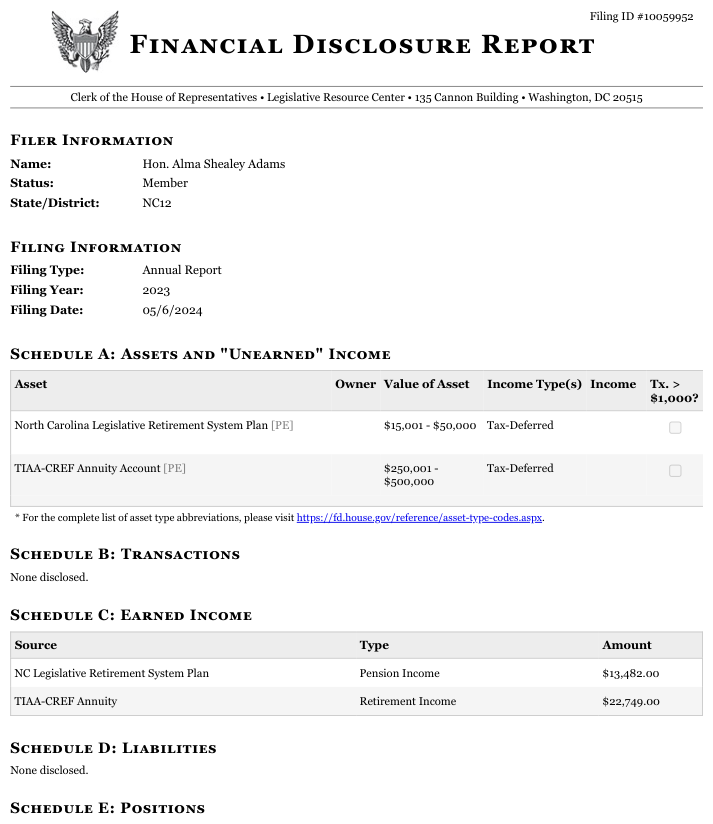
\includegraphics[height=54mm]{slides/ftype_o.png}}}\\[0.5mm]
      {\scriptsize\color{black!60} Alma Adams, 2023 — cliquable}
    \end{column}
    \begin{column}{0.64\textwidth}
      {\footnotesize
      \textbf{Qui, quand} — chaque \textbf{membre en poste}, une fois par an,
      au printemps-été suivant l'année couverte (pics mesurés : mai, puis août
      après extension).\\[1.2mm]
      \textbf{Ce qu'il contient} — 9 sections : actifs \& revenus de placement (A),
      \textbf{transactions de l'année (B)}, salaires (C), dettes (D), postes occupés (E),
      accords (F), cadeaux (G), voyages payés (H), dons reçus (I).\\[1.2mm]
      \textbf{En chiffres} — \textbf{4\,626} dépôts (dont 2 doublons d'index) ·
      3\,903 numériques / \textbf{721 scannés} · 5 pages en médiane ·
      \textbf{31 \%} ont des transactions en Schedule B.}\\[1.5mm]
      \badge{warnorange}{le plus gros gisement hors PTR — divulgué à N+1}
    \end{column}
  \end{columns}
\end{frame}

% ── H8c · Surprise : Schedule B dans les annuels ── (Pelosi, repris S1S2)
\begin{frame}{Surprise — les annuels contiennent des transactions}
  \centering
  \badge{warnorange}{type O — Annual Report 2015, Nancy Pelosi}\\[2mm]
  \fcolorbox{black!25}{white}{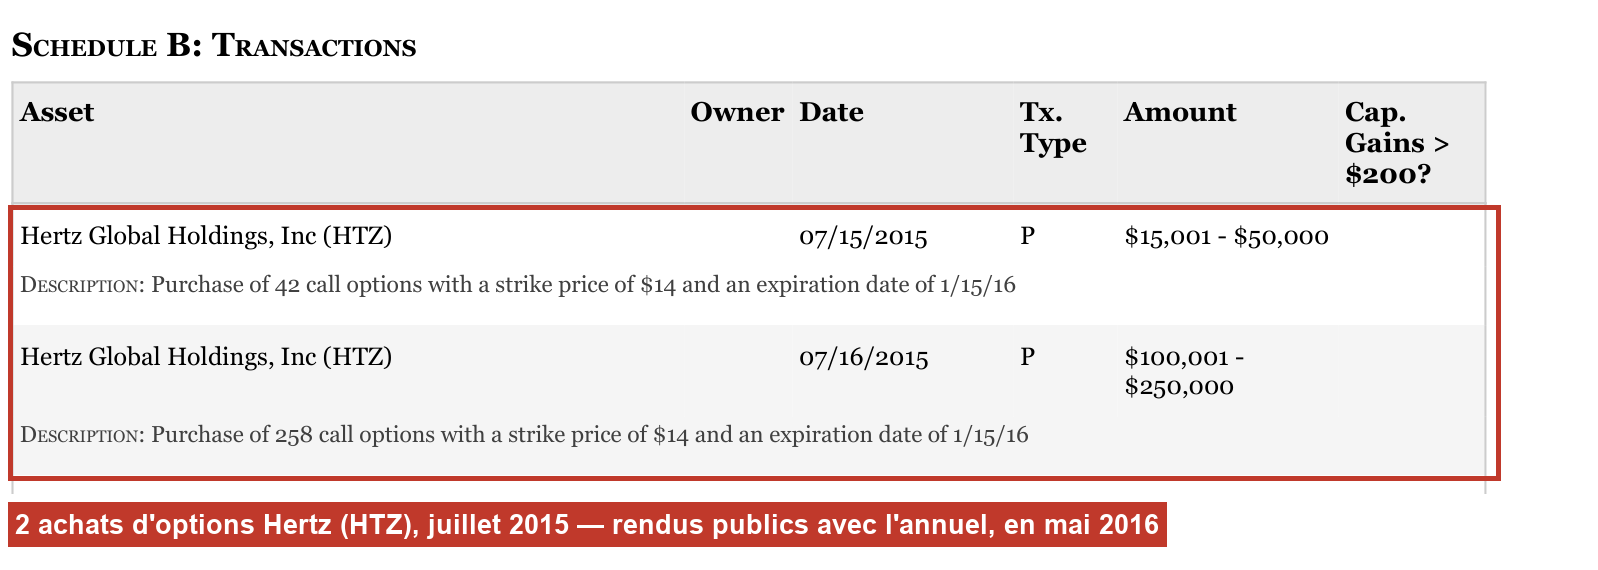
\includegraphics[width=0.80\textwidth]{slides/fig_pelosi_schedb.png}}\\[1.5mm]
  {\footnotesize la \textbf{Schedule B} d'un rapport annuel \textbf{récapitule les trades
   de l'année} — mais divulgués \textbf{un an après}. Les a-t-on déjà, au fil de l'eau,
   par les PTR ? \emph{(mesuré : slide suivante)} \;
   {\scriptsize\color{black!60}\href{https://disclosures-clerk.house.gov/public_disc/financial-pdfs/2015/10010857.pdf}{ouvrir ce rapport}}}
\end{frame}

% ── H8d · Que rate-t-on ? ── (entonnoir V1 recalculé fig_house_entonnoir_schedb ; O4 = 83,7 %)
\begin{frame}{Que rate-t-on dans ces Schedule B ? (mesuré)}
  \centering
  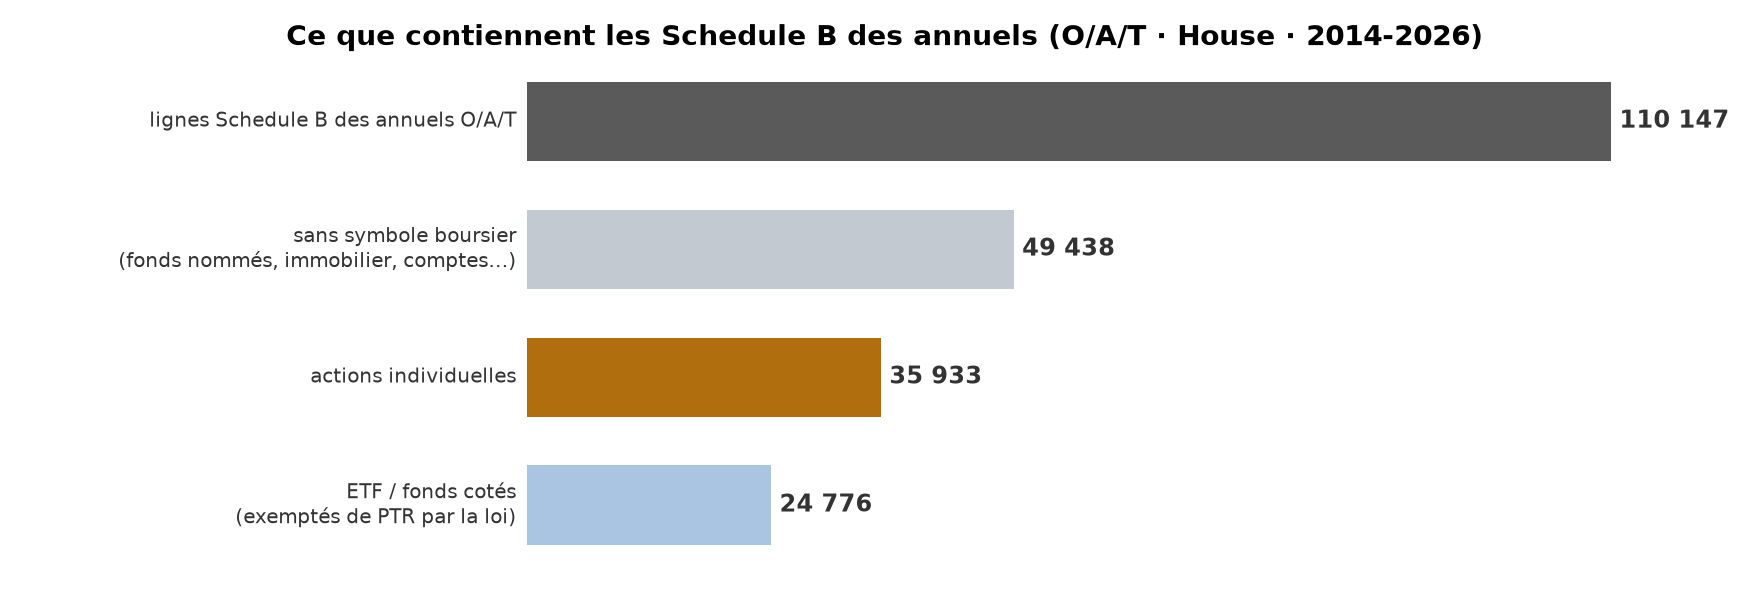
\includegraphics[width=0.80\textwidth]{fig_house_entonnoir_schedb.png}\\[1.5mm]
  \begin{columns}[c]
    \begin{column}{0.57\textwidth}
      {\footnotesize \textbf{45 \%} des lignes n'ont \emph{aucun} ticker (fonds nommés,
      immobilier, comptes) ; parmi les \textbf{actions},
      \badge{okgreen}{83,7 \% déjà en PTR} (validation O4)}
    \end{column}
    \begin{column}{0.41\textwidth}
      {\scriptsize\color{black!60} les ETF / fonds cotés ne sont pas dans les PTR car la
      \textbf{loi les en exempte} (« excepted investment funds ») — pas parce qu'on les rate}
    \end{column}
  \end{columns}
\end{frame}

% ── H8e · Ce qu'on en a fait ── (bilan : Schedule B numériques + OCR B3)
\begin{frame}{Ce qu'on en a fait — le patrimoine entièrement récupéré}
  \centering
  \begin{columns}[T]
    \begin{column}{0.49\textwidth}
      \colorbox{okgreen!12}{\parbox[t][22mm][t]{\dimexpr\linewidth-8pt}{\vspace{1mm}
        {\color{okgreen}\footnotesize\textbf{✓ Schedule B numériques — industrialisés}}\\[0.8mm]
        {\scriptsize \textbf{110\,147} transactions de contexte (fd\_O/A/T) extraites —
         table séparée, flag « divulgation annuelle »}}}\\[2mm]
      \colorbox{okgreen!12}{\parbox[t][22mm][t]{\dimexpr\linewidth-8pt}{\vspace{1mm}
        {\color{okgreen}\footnotesize\textbf{✓ Rapports scannés — OCRisés (B3)}}\\[0.8mm]
        {\scriptsize \textbf{556} documents H/T/O papier lus → \textbf{15\,489}
         holdings de plus ; là où vivaient les vieilles actions manquantes}}}
    \end{column}
    \begin{column}{0.49\textwidth}
      \colorbox{grisC!10}{\parbox[t][22mm][t]{\dimexpr\linewidth-8pt}{\vspace{1mm}
        {\color{grisC}\footnotesize\textbf{· Fonds sans ticker (49\,438)}}\\[0.8mm]
        {\scriptsize « vue patrimoine » — appariement par \emph{nom} d'actif =
         suite (priorité basse)}}}\\[2mm]
      \colorbox{grisC!10}{\parbox[t][22mm][t]{\dimexpr\linewidth-8pt}{\vspace{1mm}
        {\color{grisC}\footnotesize\textbf{· Blind trusts (23 docs)}}\\[0.8mm]
        {\scriptsize analysés à part · \textbf{jamais dans le signal} (non dirigé par l'élu)}}}
    \end{column}
  \end{columns}
  \vspace{2.5mm}
  \colorbox{alertred}{\parbox{0.9\textwidth}{\footnotesize\color{white}\centering
    dans tous les cas : \textbf{jamais dans le backtest daté} — divulgation médiane
    \textbf{371 j} après le trade (vs \textbf{28 j} via PTR) → de la complétude, pas du signal}}
\end{frame}

% ── AN5 · A ── (recensement V1 : 2 305 ; ledger : 1 870/433)
\begin{frame}{À tout moment — \texttt{A}, l'amendement qui corrige un dépôt}
  \begin{columns}[c]
    \begin{column}{0.34\textwidth}\centering
      \href{https://disclosures-clerk.house.gov/public_disc/financial-pdfs/2023/10062190.pdf}{\fcolorbox{black!30}{white}{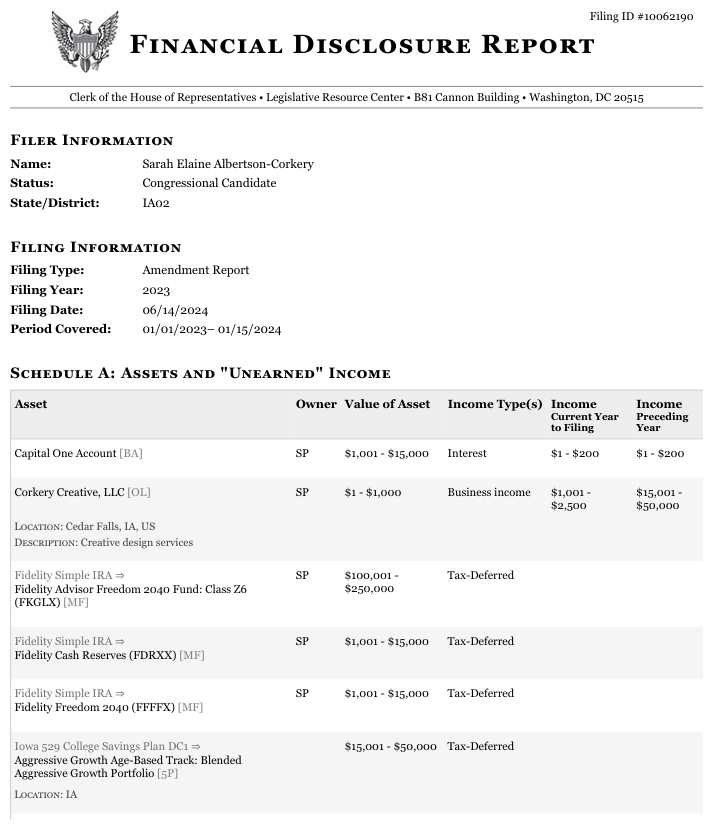
\includegraphics[height=54mm]{slides/ftype_a.png}}}\\[0.5mm]
      {\scriptsize\color{black!60} Sarah Albertson-Corkery, 2023 — cliquable}
    \end{column}
    \begin{column}{0.64\textwidth}
      {\footnotesize
      \textbf{Qui, quand} — n'importe quel déposant qui \textbf{corrige un dépôt
      antérieur} (annuel, candidat, sortie…) — le document corrigé est re-déposé
      en entier.\\[1.2mm]
      \textbf{Ce qu'il contient} — les sections \textbf{du document qu'il corrige} :
      un amendement d'annuel a une Schedule B, un amendement de candidat n'en a pas
      (mesuré : 26 \% avec transactions).\\[1.2mm]
      \textbf{En chiffres} — \textbf{2\,305} dépôts (72 \% membres,
      le reste candidats) · 5 pages en médiane.\\[1.2mm]
      \textbf{Piège mesuré} — l'amendement \textbf{répète} les trades de l'annuel
      qu'il corrige (ex. Pelosi 2014 : le même trade apparaît 3 fois O+A+A) —
      la dédup V1 les compte une fois.}\\[1.5mm]
      \badgel{grisC!30}{rien de neuf en soi : suit le sort du document corrigé}
    \end{column}
  \end{columns}
\end{frame}

% ── AN4 · T ── (recensement V1 : 394 ; ledger : 291/102)
\begin{frame}{La sortie — \texttt{T}, la photo finale du portefeuille}
  \begin{columns}[c]
    \begin{column}{0.34\textwidth}\centering
      \href{https://disclosures-clerk.house.gov/public_disc/financial-pdfs/2023/10050798.pdf}{\fcolorbox{black!30}{white}{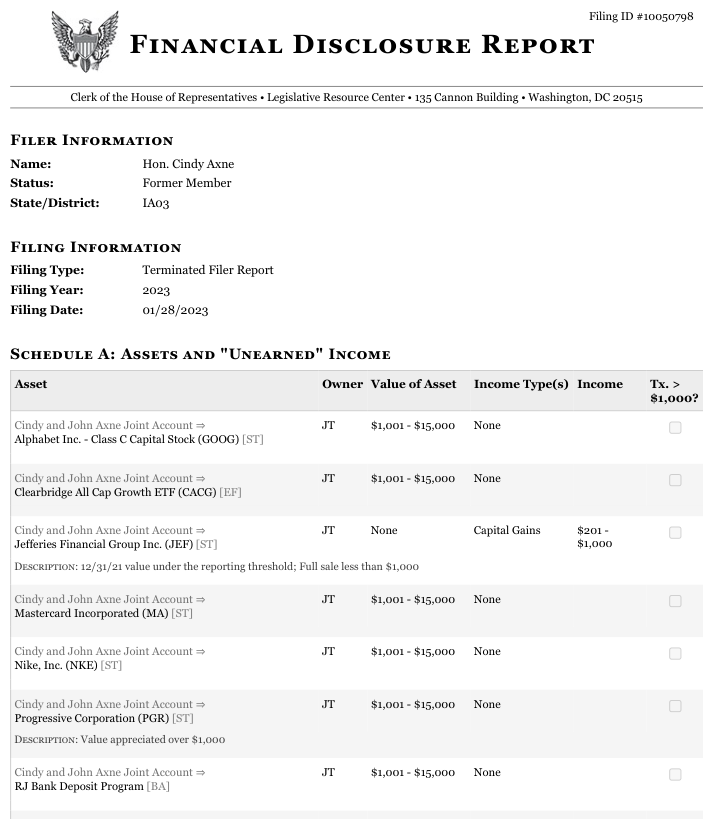
\includegraphics[height=54mm]{slides/ftype_t.png}}}\\[0.5mm]
      {\scriptsize\color{black!60} Cindy Axne, départ de la Chambre, 2023 — cliquable}
    \end{column}
    \begin{column}{0.64\textwidth}
      {\footnotesize
      \textbf{Qui, quand} — un membre qui \textbf{quitte la Chambre} (fin de mandat,
      démission) — déposé surtout en janvier-février suivant le départ (mesuré).\\[1.2mm]
      \textbf{Ce qu'il contient} — le formulaire complet du rapport annuel
      (9 sections, \textbf{dont les transactions (B)}) sur l'année partielle
      jusqu'au départ. \textbf{28 \%} en contiennent.\\[1.2mm]
      \textbf{En chiffres} — \textbf{394} dépôts (99 \% membres, dont 1 doublon d'index) ·
      291 numériques / 102 scannés · 5 pages en médiane.\\[1.2mm]
      \textbf{Exemple réel} — la sortie d'Eric Cantor (2014) contient des achats
      d'ETF jamais déposés en PTR — ils font partie des 173 trades « annuel-seul ».}\\[1.5mm]
      \badge{dataC}{la photo de SORTIE : l'autre borne du contrôle H + P ⊇ T}
    \end{column}
  \end{columns}
\end{frame}

% ── H8b · Le bilan démographique H/T ── (§15 du notebook ; D-1 98,1 · D-2 81,4 · D-3 281 = 258+23)
\begin{frame}{H = 395, T = 394 — et pourtant il ne « reste » pas 1}
  \centering
  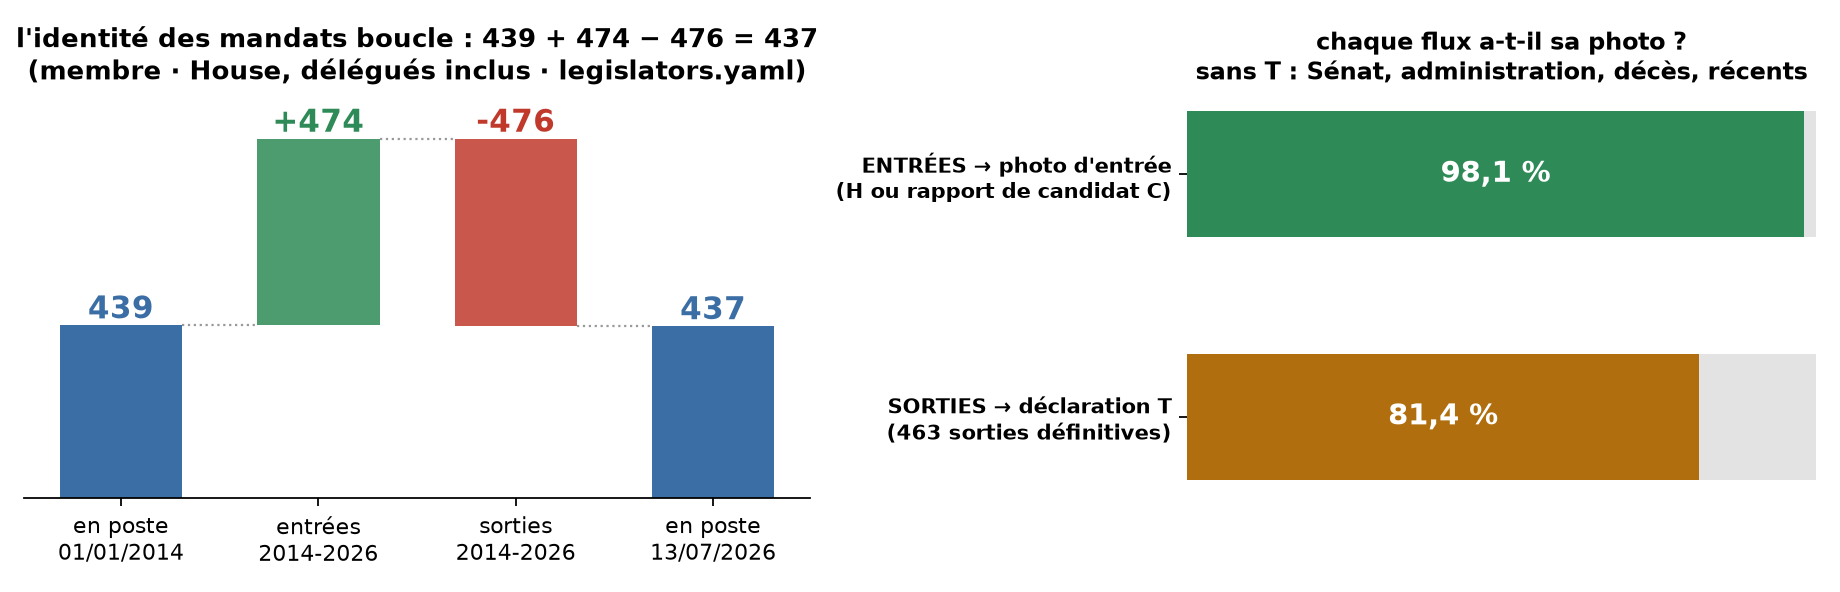
\includegraphics[width=0.97\textwidth]{fig_house_flux.png}\\[1.5mm]
  \begin{columns}[T]
    \begin{column}{0.55\textwidth}
      {\footnotesize soustraire H et T n'a pas de sens : les \textbf{439 déjà en poste}
      en 2014 n'ont jamais déposé de H, 18 \% des entrants sont \textbf{dispensés de H
      par leur rapport de candidat C}, et 18,6 \% des sortants ne déposent pas de T
      (bascule au \textbf{Sénat}, administration, décès, départs trop récents).}
    \end{column}
    \begin{column}{0.43\textwidth}
      \badge{helec}{il en reste 437 (431 votants)}\\[1.5mm]
      {\scriptsize\color{black!60} et seuls \textbf{106} membres ont les DEUX photos
       (H et T) : c'est le vivier de la cohorte de cohérence de l'acte 6 —
       45 exploitables en électronique}
    \end{column}
  \end{columns}
\end{frame}

\section{Les documents — lisible ou scanné, le préfixe du DocID le dit}

% ── H9 · La nomenclature des préfixes ── (02_ledger_docs.csv : croisé 1er car. × type)
\begin{frame}{Le \texttt{DocID} (1/4) — son premier chiffre annonce la nature du PDF}
  \centering
  \begin{columns}[T]
    \begin{column}{0.46\textwidth}
      {\footnotesize\setlength{\tabcolsep}{5pt}
      \begin{tabular}{c l l}
        \toprule
        préfixe & types & nature du PDF \\
        \midrule
        \co{1…} & C·O·H·T·A & \textcolor{helec}{\textbf{numérique}} \\
        \co{2…} & \textcolor{helec}{\textbf{P}} & \textcolor{helec}{\textbf{numérique}} \\
        \co{3…} & X & numérique \\
        \co{4…} & D & numérique \\
        \co{6xxx}/\co{7…} & W & (papier admin) \\
        \midrule
        \co{8…} / \co{9…} & \textbf{tous} & \textcolor{black!60}{\textbf{scanné} (image)} \\
        \bottomrule
      \end{tabular}}\\[2mm]
      {\scriptsize\color{black!55} chaque type \emph{numérique} a SON préfixe —
       le formulaire en ligne le génère}
    \end{column}
    \begin{column}{0.52\textwidth}
      \centering
      \resizebox{0.96\linewidth}{!}{%
      \begin{tikzpicture}[node distance=8mm]
        \node[step=helec, text width=3.1cm] (d) {le \co{DocID} du dépôt\\[1mm]\co{20024277}};
        \node[step=grisC, text width=4.6cm, below=6mm of d] (u)
          {une URL de PDF\\[1mm]{\scriptsize\ttfamily …/ptr-pdfs/2024/20024277.pdf}};
        \node[step=helec, fill=helec!16, text width=3.6cm, below left=6mm and -14mm of u] (lis)
          {\textbf{lisible} (texte)\\{\scriptsize DocID en \co{2…}}};
        \node[step=hocr, fill=hocr!40, text width=3.6cm, below right=6mm and -14mm of u] (sc)
          {\textbf{scanné} (image)\\{\scriptsize DocID en \co{8…}/\co{9…}}};
        \draw[arr] (d) -- (u);
        \draw[arr] (u.south) -- (lis.north);
        \draw[arr] (u.south) -- (sc.north);
      \end{tikzpicture}}\\[1.5mm]
      {\scriptsize\color{black!55} deux règles d'URL, apprises en ouvrant les documents :
       \co{P} → \co{…/ptr-pdfs/…} · tous les autres → \co{…/financial-pdfs/…}}
    \end{column}
  \end{columns}
\end{frame}

% ── H9a · Un PTR lisible ── (fig_ptr_digital, Yarmuth ; repris S1S2)
\begin{frame}{Le \texttt{DocID} en \texttt{2…} — à quoi ressemble un PTR lisible}
  \begin{columns}[T]
    \begin{column}{0.55\textwidth}\centering
      \fcolorbox{helec}{white}{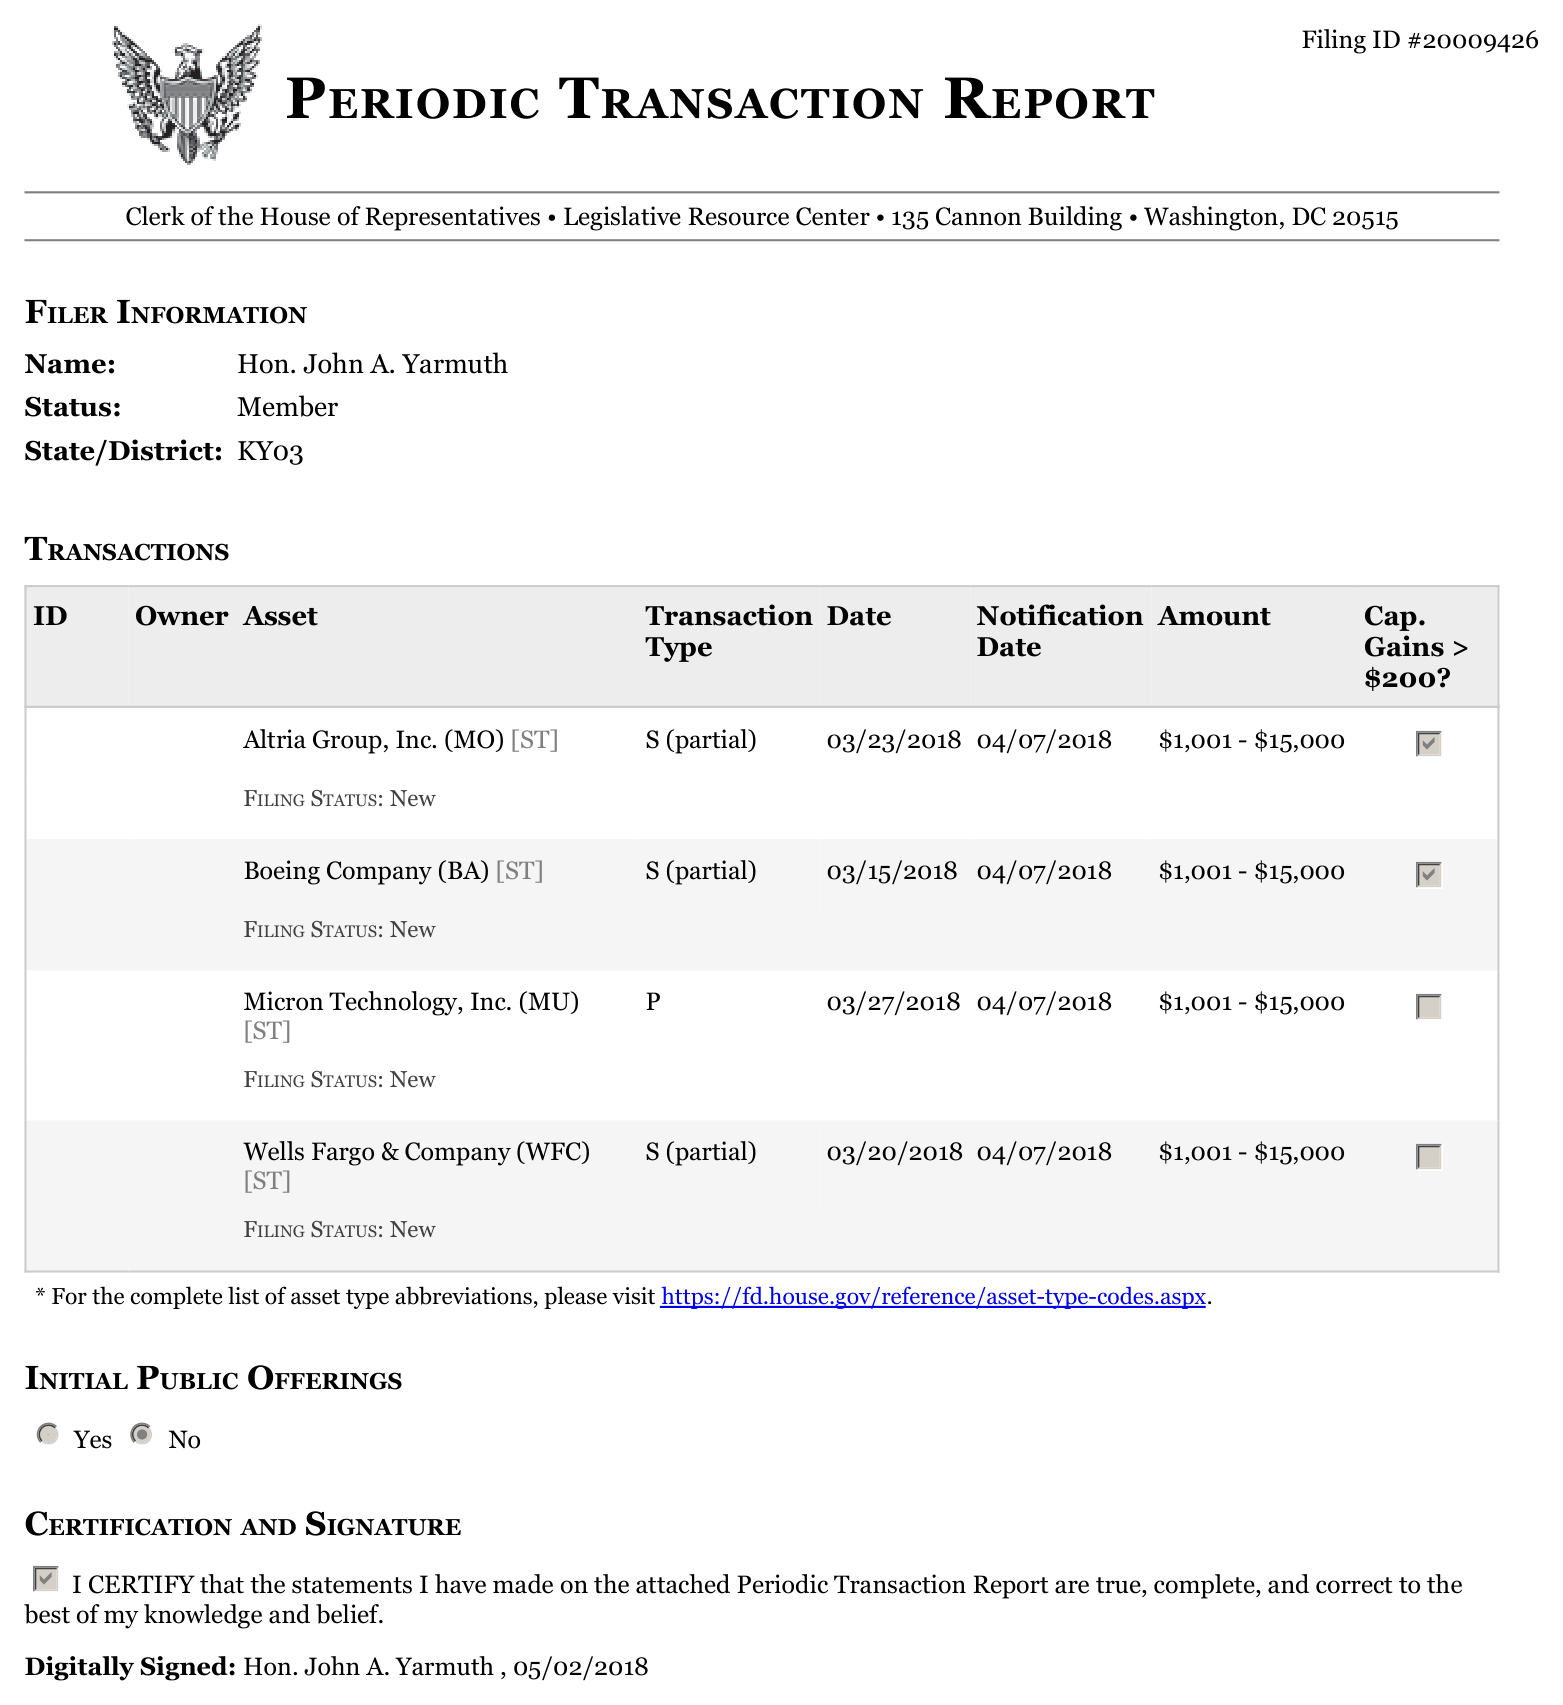
\includegraphics[height=64mm]{slides/fig_ptr_digital.png}}\\[0.5mm]
      {\scriptsize\color{black!60} PTR électronique complet (Hon. John A. Yarmuth, KY03)}
    \end{column}
    \begin{column}{0.43\textwidth}
      \badge{helec}{DocID en \co{2…} → PDF lisible}\\[3mm]
      {\footnotesize
      · un PDF \textbf{avec couche texte} : lisible machine\\[1.5mm]
      · le ticker imprimé \textbf{entre parenthèses} : \co{(BA)}, le type d'actif
        entre crochets : \co{[ST]}\\[1.5mm]
      · deux dates par ligne (trade / notification) + fourchette de montant\\[1.5mm]
      · lisible… mais pas si régulier : \textcolor{alertred}{le défi} en face}
    \end{column}
  \end{columns}
\end{frame}

% ── H9b · Le défi de l'extraction ── (fig_ptr_multiligne, Gibbs ; V1 : 119 montants recollés)
\begin{frame}{Le défi — un PDF lisible n'est pas un tableau régulier}
  \begin{columns}[T]
    \begin{column}{0.60\textwidth}\centering
      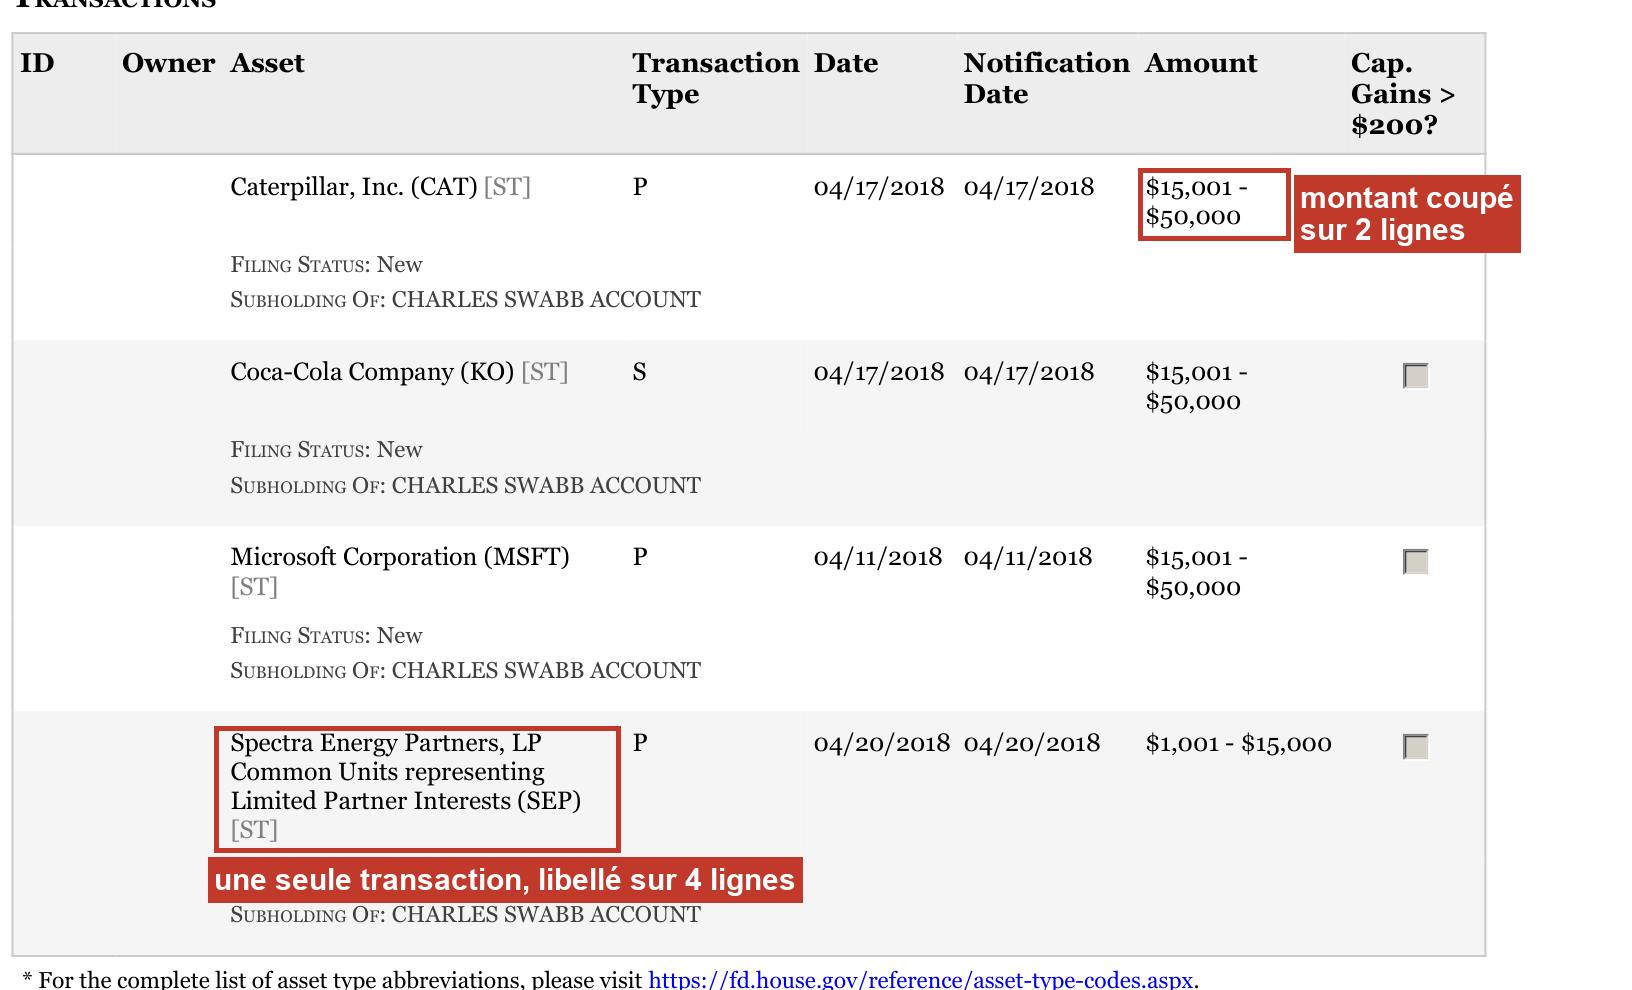
\includegraphics[width=\linewidth]{slides/fig_ptr_multiligne.png}\\[0.5mm]
      {\scriptsize\color{black!60} extrait réel (Hon.\ Bob Gibbs, OH07) — cadres ajoutés}
    \end{column}
    \begin{column}{0.38\textwidth}
      {\footnotesize
      · le \textbf{montant} déborde sur la ligne suivante (\co{\$15,001 -} puis
        \co{\$50,000})\\[1.2mm]
      · le \textbf{libellé} d'un actif court sur \textbf{4 lignes}\\[1.2mm]
      · un découpage ligne à ligne raterait la moitié}\\[2mm]
      \colorbox{helec}{\parbox{0.95\linewidth}{\footnotesize\color{white}\centering
        → le parseur V1 \textbf{reconstruit} chaque\\ transaction (recollage des
        lignes coupées)}}\\[1.5mm]
      {\scriptsize\color{black!60} montant recousu sur 2 lignes : \textbf{119} cas
       (le parseur gère le reste nativement)}
    \end{column}
  \end{columns}
\end{frame}

% ── H9c · Un PTR scanné (3 formes) ── (V1 : 105 074 txns OCR = 65 % du signal)
\begin{frame}{Le \texttt{DocID} en \texttt{8…}/\texttt{9…} — à quoi ressemble un PTR scanné}
  \centering
  {\footnotesize un scan n'est pas du texte, c'est une \textbf{image} — sous trois formes
   (pages réelles) :}\\[2.5mm]
  \begin{columns}[T]
    \begin{column}{0.37\textwidth}\centering
      \fcolorbox{black!30}{white}{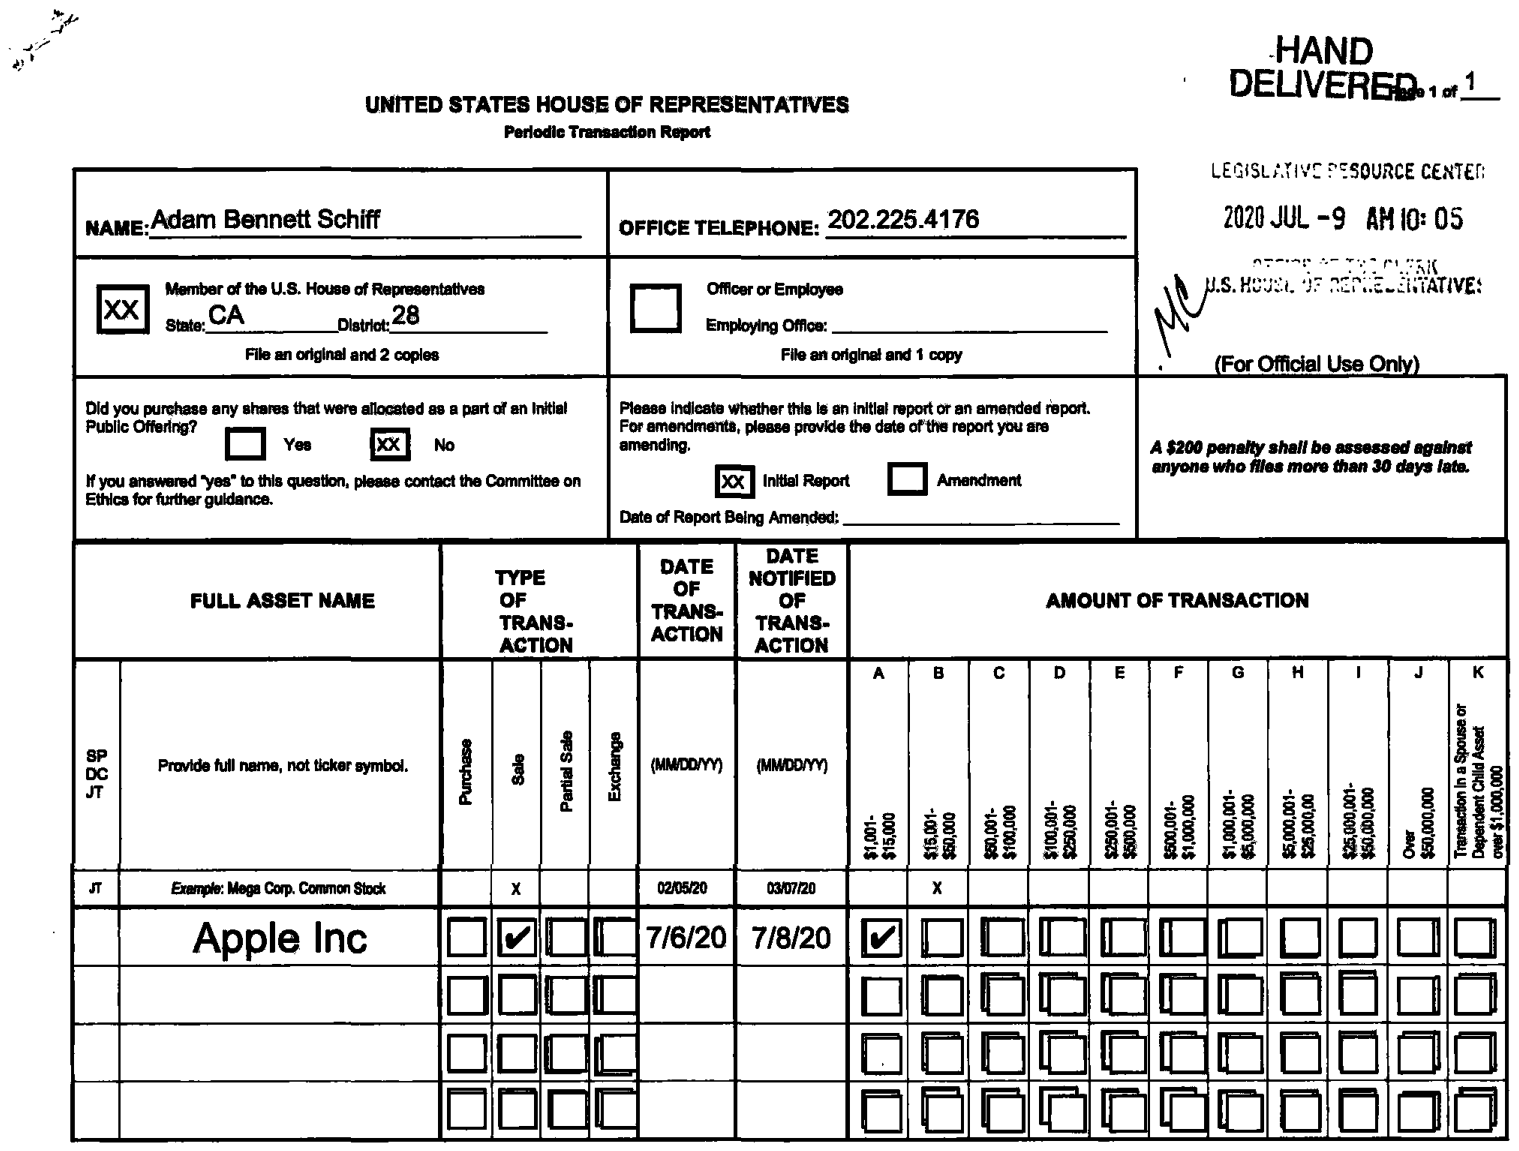
\includegraphics[height=34mm]{slides/scan_full_droit.png}}\\[1.2mm]
      {\footnotesize\textbf{Tapé, droit}}\\[0.3mm]{\scriptsize dactylographié, lisible tel quel}
    \end{column}
    \begin{column}{0.21\textwidth}\centering
      \fcolorbox{black!30}{white}{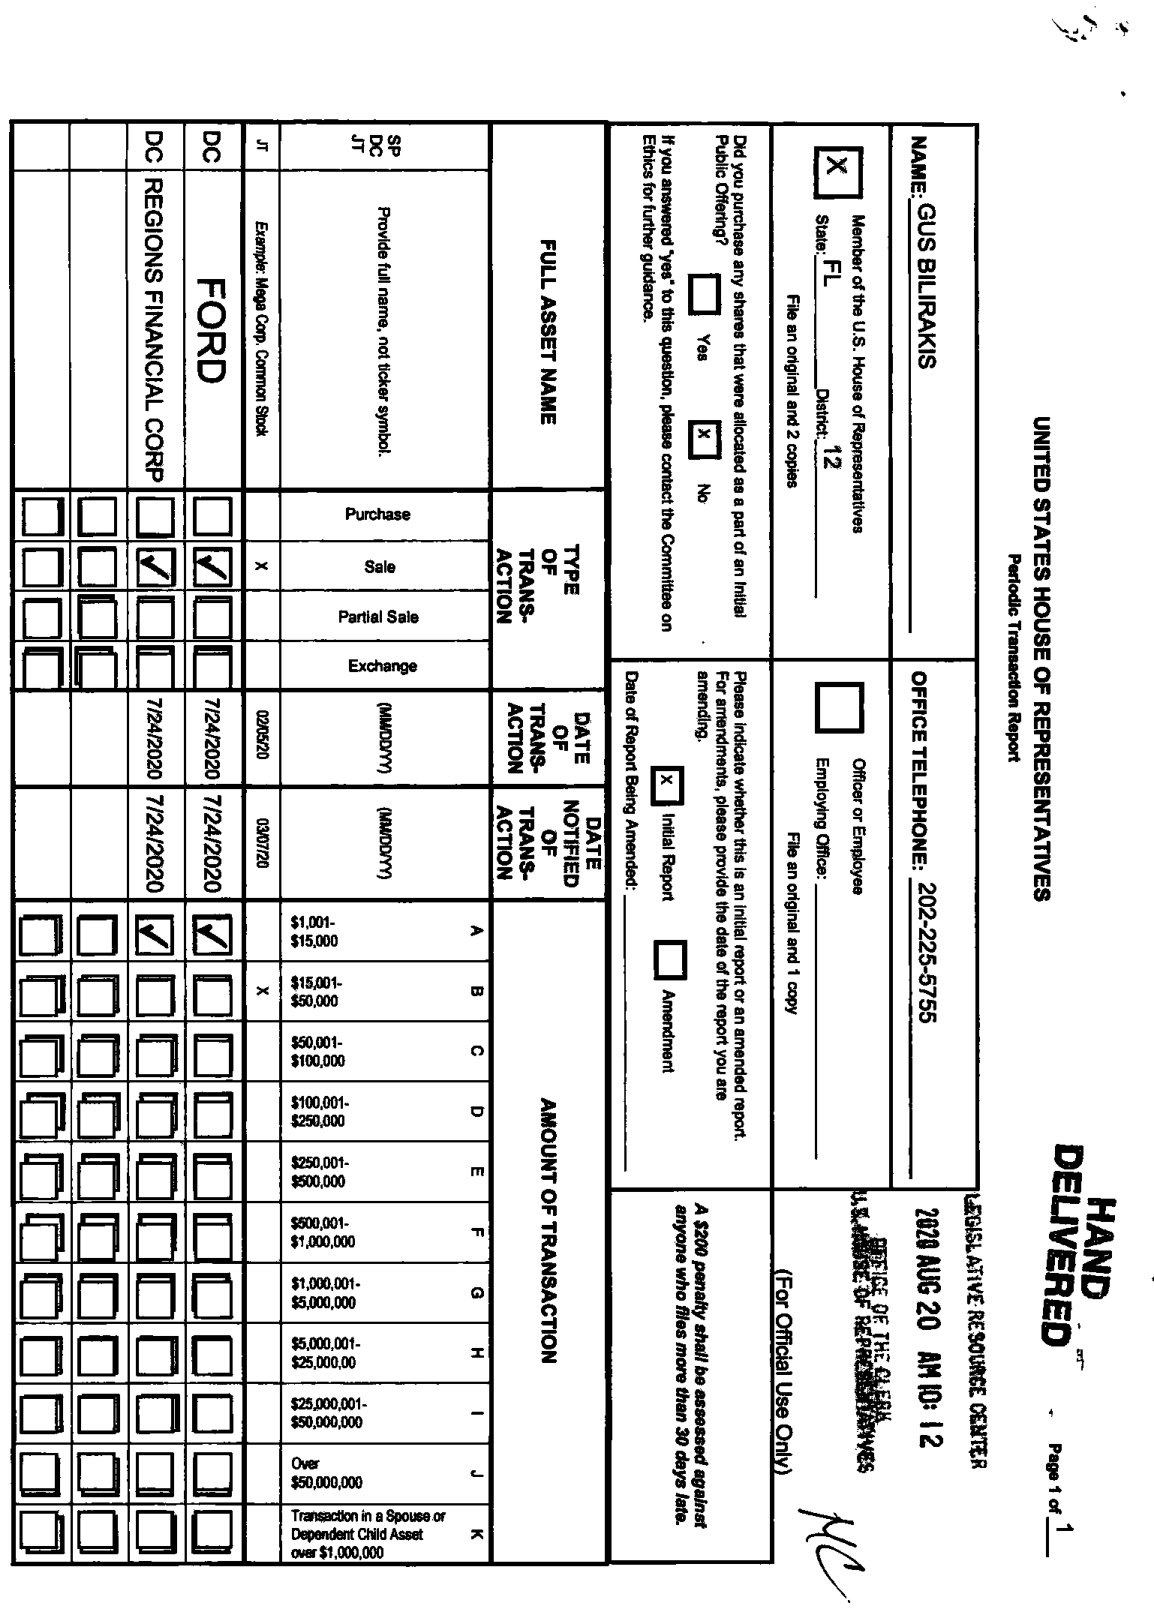
\includegraphics[height=34mm]{slides/scan_full_couche.png}}\\[1.2mm]
      {\footnotesize\textbf{Tapé, couché}}\\[0.3mm]{\scriptsize tourné à 90°\\(le plus courant)}
    \end{column}
    \begin{column}{0.37\textwidth}\centering
      \fcolorbox{black!30}{white}{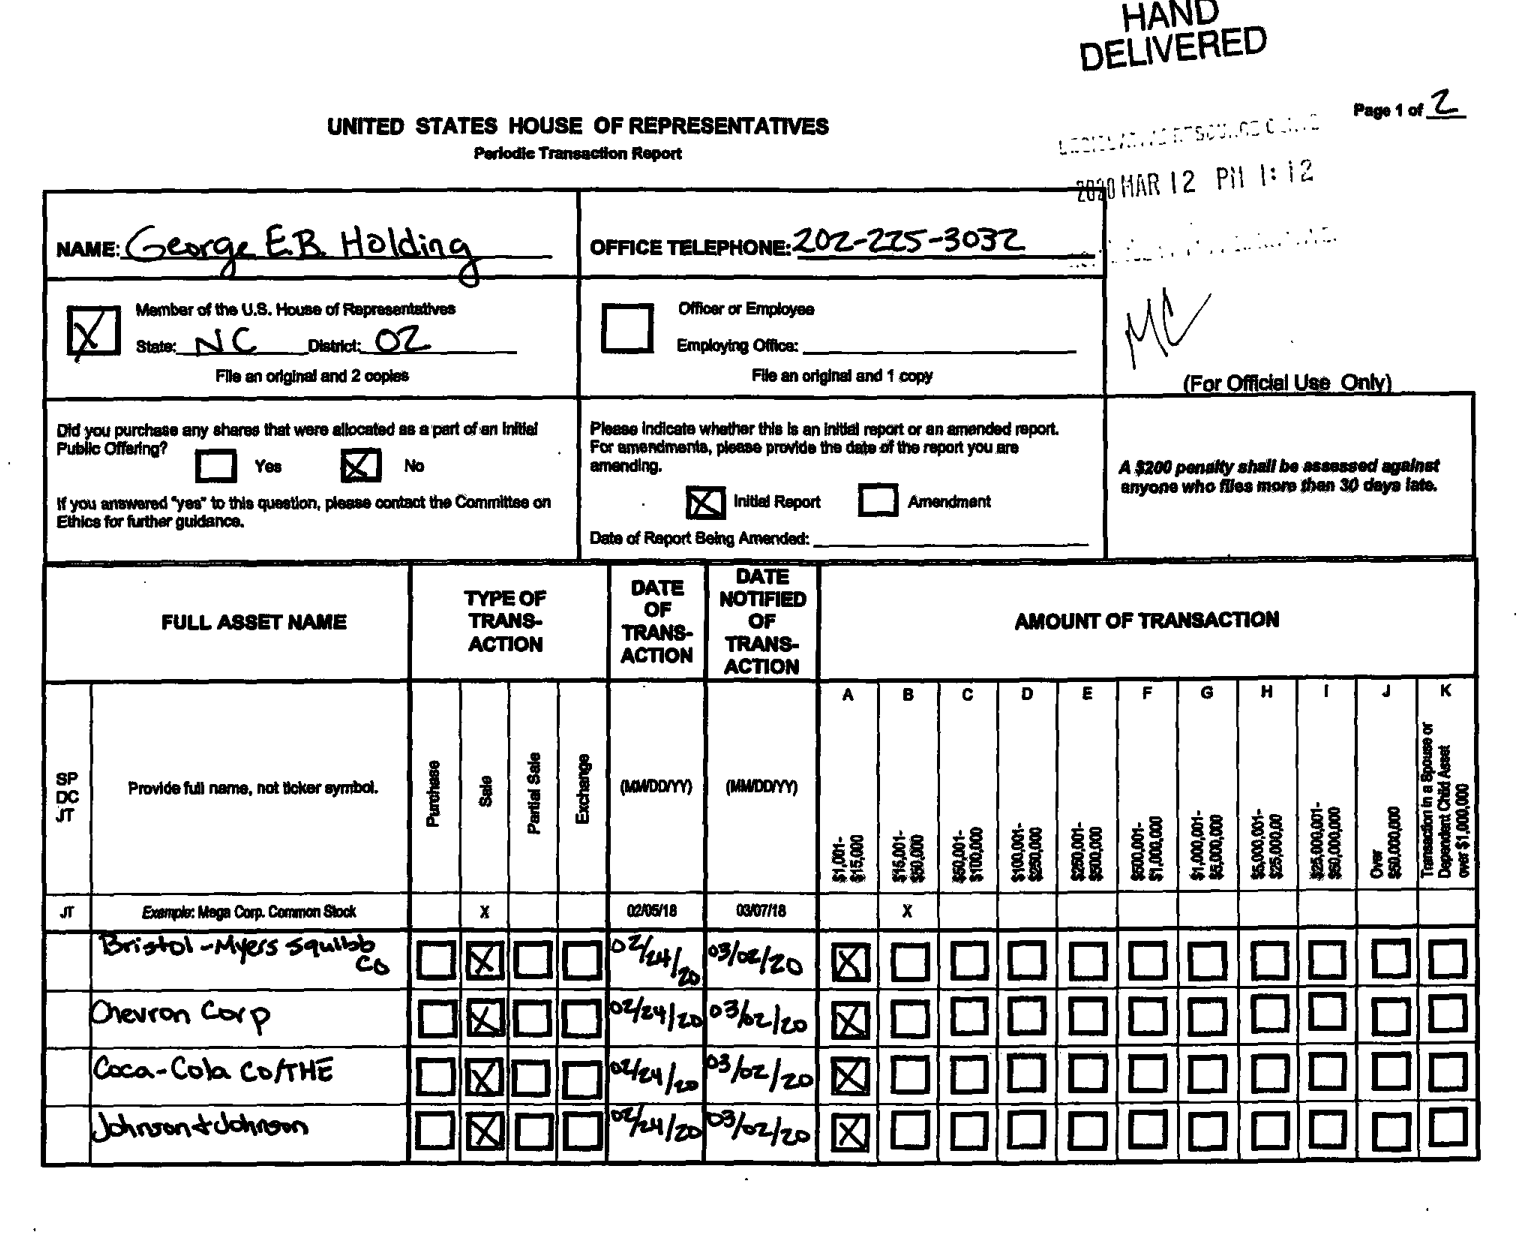
\includegraphics[height=34mm]{slides/scan_full_manuscrit.png}}\\[1.2mm]
      {\footnotesize\textbf{Manuscrit}}\\[0.3mm]{\scriptsize rempli \textbf{à la main}, en cursif}
    \end{column}
  \end{columns}
  \vspace{2mm}
  \badgel{hocr}{105\,074 transactions lues par OCR — 65 \% du signal PTR}\quad
  {\scriptsize\color{black!60} Claude Vision (cache hérité + B3)}
\end{frame}

% ── H10 · La preuve : matrice préfixe × contenu ── (V1_House.ipynb §5.2 ; validation L4=0)
\begin{frame}{Le \texttt{DocID} (2/4) — le préfixe dit-il vrai ? Vérifié sur 24\,078 PDF}
  \centering
  {\footnotesize deux définitions \textbf{indépendantes} de « scanné », confrontées
   document par document :}\\[1mm]
  {\footnotesize la \textbf{métadonnée} (préfixe du DocID) \emph{vs} la \textbf{réalité
   physique} (le PDF a-t-il une couche texte ? — \co{pdfplumber})}\\[3.5mm]
  {\normalsize\setlength{\tabcolsep}{10pt}\renewcommand{\arraystretch}{1.35}
  \begin{tabular}{l cc}
    \toprule
    & PDF \textbf{avec} couche texte & PDF \textbf{sans} couche texte \\
    \midrule
    préfixe numérique (\co{1}/\co{2}/\co{3}/\co{4}) &
      \textcolor{okgreen}{\textbf{20\,821}} & \textcolor{alertred}{\textbf{0}} \\
    préfixe scanné (\co{8}/\co{9}) &
      \textcolor{alertred}{\textbf{0}} & \textcolor{okgreen}{\textbf{3\,257}} \\
    \bottomrule
  \end{tabular}}\\[4mm]
  \badge{okgreen}{0 désaccord sur 24\,078 documents — validation L4}\\[2mm]
  {\scriptsize\color{black!60} périmètre : PDF en cache, types P·C·H·O·T·A · 2014-2026 —
   le tri lisible/scanné n'est \textbf{pas une hypothèse}, c'est une \textbf{mesure} ;
   l'ancien pipeline, lui, ne regardait que le contenu (fragile aux PDF mal formés)}
\end{frame}

% ── H11 · Proportions élec/scanné par type ── (02_ledger_docs.csv ; fig scans par année)
\begin{frame}{Le \texttt{DocID} (3/4) — combien de scannés, réellement ?}
  \begin{columns}[T]
    \begin{column}{0.40\textwidth}
      {\footnotesize\setlength{\tabcolsep}{4.5pt}
      \begin{tabular}{l r rr}
        \toprule
        type & docs & \multicolumn{1}{c}{élec} & \multicolumn{1}{c}{scanné} \\
        \midrule
        \textcolor{helec}{\textbf{P}} & 8\,267 & \textbf{70,7\,\%} & \textbf{29,3\,\%} \\
        C & 10\,116 & 84,4\,\% & 15,6\,\% \\
        O & 4\,624 & 84,4\,\% & 15,6\,\% \\
        A & 2\,303 & 81,2\,\% & 18,8\,\% \\
        H & 395 & 97,0\,\% & 3,0\,\% \\
        T & 393 & 74,0\,\% & 26,0\,\% \\
        \bottomrule
      \end{tabular}}\\[2mm]
      {\scriptsize\color{black!55} unité : document unique du ledger
       (18 DocID doublonnés inter-index comptés une fois)}
    \end{column}
    \begin{column}{0.58\textwidth}\centering
      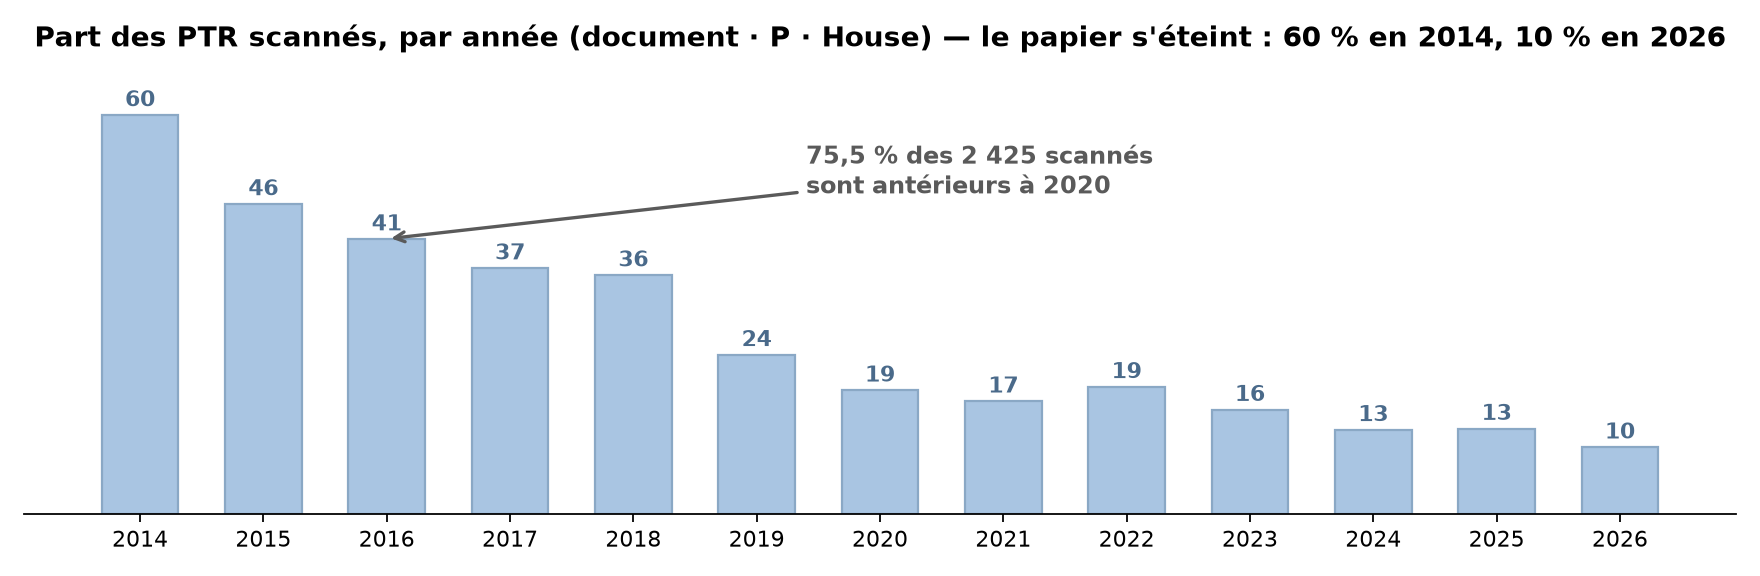
\includegraphics[width=\linewidth]{fig_house_scans_par_annee.png}\\[1.5mm]
      {\footnotesize le scan est un phénomène \textbf{2014-2019} :
       les trois quarts des PTR papier sont antérieurs à 2020 —
       le formulaire en ligne a gagné}
    \end{column}
  \end{columns}
\end{frame}

% ── H12 · Le paradoxe résolu ── (04/07_transactions : 56 002 élec + 105 074 OCR ; fig paradoxe)
\begin{frame}{Le \texttt{DocID} (4/4) — le paradoxe : 29 \% des documents, 65 \% des transactions}
  \centering
  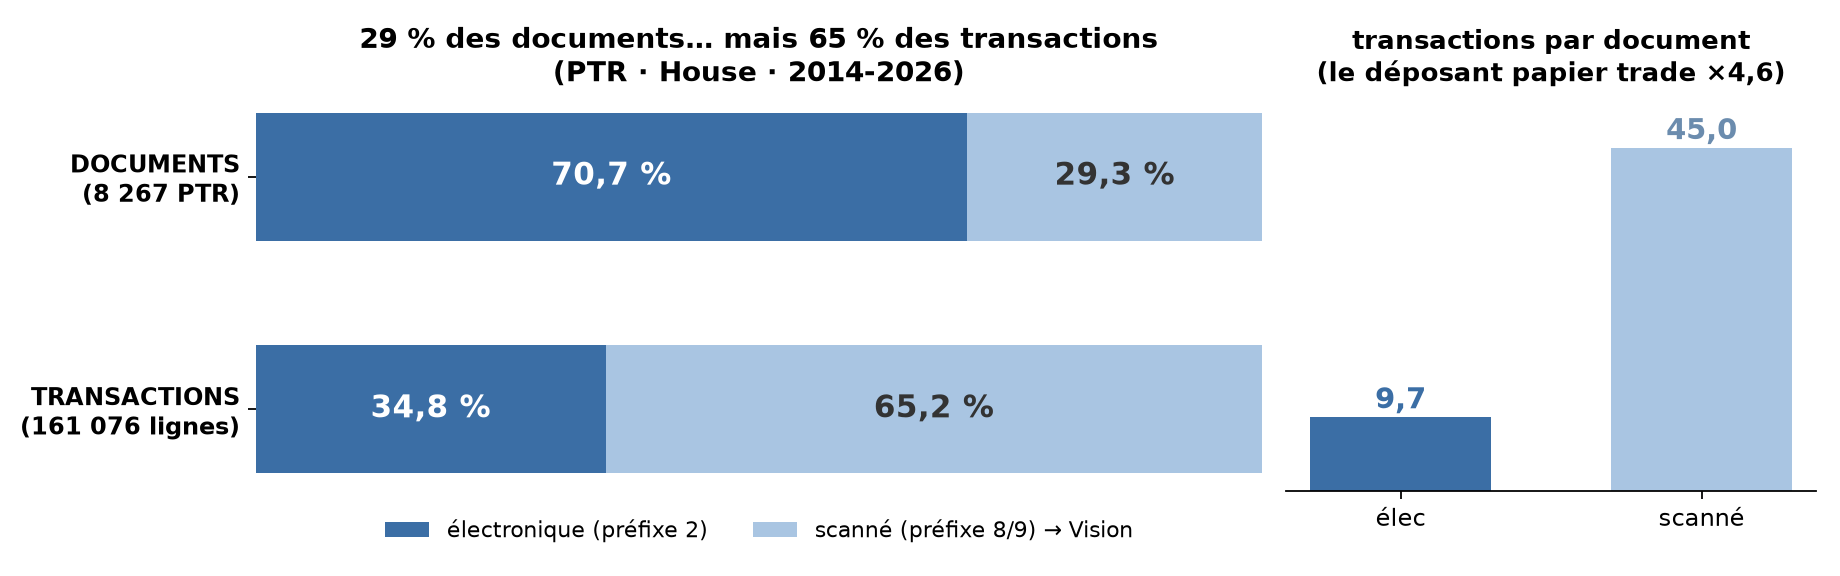
\includegraphics[width=0.86\textwidth]{fig_house_paradoxe.png}\\[1.5mm]
  \begin{columns}[T]
    \begin{column}{0.55\textwidth}
      {\footnotesize « Vision lit 65 \% de la donnée » et « 70 \% des PTR sont
      électroniques » sont \textbf{tous deux vrais} — l'unité change :
      \textbf{document} d'un côté, \textbf{transaction} de l'autre.
      Les déposants papier sont simplement les plus actifs
      (45,0 lignes par document, contre 9,7).}
    \end{column}
    \begin{column}{0.43\textwidth}
      \badge{helec}{rien de parsable ne part en OCR}\\[1.5mm]
      {\scriptsize\color{black!60} Vision ne lit QUE les 2\,425 P réellement
       scannés (préfixe 8/9, 0 désaccord de contenu) — les 5\,842 P
       électroniques sont parsés au texte}
    \end{column}
  \end{columns}
\end{frame}

\section{Rien d'oublié — la comptabilité des 35 377}

% ── N3 · La comptabilité finale ── (§18 : G-1 BLOQUANT 35 377 · G-2 18 171 · G-3 2 296 ; fig_house_compta)
\begin{frame}{Rien d'oublié — chaque dépôt a un traitement, la somme boucle}
  \centering
  
\includegraphics[width=0.88\textwidth]{fig_house_compta.png}\\[1.5mm]
  {\footnotesize \badge{okgreen}{G-1 (bloquant) : Σ = 35\,377 ✓}\;
   \badge{okgreen}{18\,171 docs → données (G-2)}\;
   \badgel{dataC!30}{\textcolor{dataC}{\textbf{14\,892 recensés, rien à extraire}}}\;
   \badgel{grisC!25}{\textcolor{grisC}{\textbf{2\,296 différés — tous tracés (G-3)}}}}\\[1mm]
  {\scriptsize\color{black!60} vert = données extraites · ocre = recensé sans donnée
   (vides, admin, blind trusts) · gris = différé/exclu avec raison écrite —
   table nominative : \co{10\_comptabilite\_traitement.csv}}
\end{frame}

% ── N4 · Ce que ça a livré ── (04/05/07/08/09 : 280 677 txns + 214 104 holdings)
\begin{frame}{Ce que ces documents ont livré}
  \centering
  \tuile{helec}{280\,677}{transactions\\extraites au total}\hfill
  \tuile{dataC}{214\,104}{holdings\\(photos de patrimoine)}\hfill
  \tuile{okgreen}{161\,076}{= le SIGNAL\\(PTR datés au trade)}\hfill
  \tuile{grisC}{119\,601}{= le CONTEXTE\\(Schedule B des annuels)}\\[4mm]
  {\footnotesize\setlength{\tabcolsep}{8pt}
  \begin{tabular}{l r l r}
    \toprule
    \textbf{transactions} & & \textbf{holdings} & \\
    \midrule
    PTR électroniques & 56\,002 & Schedule A électroniques & 198\,615 \\
    PTR scannés (OCR) & 105\,074 & Schedule A scannés (OCR B3) & 15\,489 \\
    Schedule B électroniques (O/A/T) & 110\,147 & & \\
    Schedule B scannés (OCR B3) & 9\,454 & & \\
    \bottomrule
  \end{tabular}}\\[2.5mm]
  {\scriptsize\color{black!60} seul le signal (PTR) est tradable — le contexte sert
   aux contrôles de cohérence de l'acte 6}
\end{frame}

\section{Les portefeuilles se recoupent — entrée + transactions ⊇ sortie}

% ── H13 · L'idée : H + ΣP ⊇ T, contrôlé par O/A ── (V1_House.ipynb §11)
\begin{frame}{Le contrôle final — la chronologie d'un mandat doit se recouper}
  \centering
  {\footnotesize chaque élu déclare sa \textbf{photo d'entrée} (H), ses
   \textbf{transactions} (P), des \textbf{bilans annuels} (O, corrigés par A),
   et sa \textbf{photo de sortie} (T) : quatre déclarations \textbf{indépendantes}
   du même portefeuille}\\[4mm]
  \resizebox{0.97\textwidth}{!}{%
  \begin{tikzpicture}[node distance=8mm]
    \node[step=okgreen, text width=2.9cm, minimum height=1.55cm, font=\footnotesize] (h)
      {\textbf{ENTRÉE}\\rapport \co{H}\\{\scriptsize Schedule A : ce qu'il détient}};
    \node[step=helec, text width=3.3cm, minimum height=1.55cm, font=\footnotesize, right=of h] (p)
      {\textbf{+ les transactions}\\les \co{P} du mandat\\{\scriptsize achats / ventes datés}};
    \node[step=dataC, text width=3.0cm, minimum height=1.55cm, font=\footnotesize, right=of p] (o)
      {\textbf{contrôles en route}\\annuels \co{O} (+ \co{A})\\{\scriptsize une photo par année}};
    \node[step=grisC, fill=dataC!14, draw=dataC, text width=2.9cm, minimum height=1.55cm, font=\footnotesize, right=of o] (t)
      {\textbf{SORTIE}\\rapport \co{T}\\{\scriptsize Schedule A : ce qu'il emporte}};
    \draw[-{Latex[length=2.6mm]}, line width=1pt] (h) -- (p);
    \draw[-{Latex[length=2.6mm]}, line width=1pt] (p) -- (o);
    \draw[-{Latex[length=2.6mm]}, line width=1pt] (o) -- (t);
    \node[below=5mm of o, font=\small\bfseries, color=alertred]
      {si notre collecte rate des transactions, l'identité casse — c'est un détecteur de trous};
  \end{tikzpicture}}
  \\[4.5mm]
  {\footnotesize\centering
   \textbf{H} $+$ \textbf{$\Sigma$ P} $\supseteq$ \textbf{T}\quad — testé position par
   position (ticker), membre par membre}
\end{frame}

% ── H14 · Le moteur : créer le portefeuille d'un membre ── (adaptation « positions » de la slide moteur S3)
\begin{frame}{Le moteur — reconstruire le portefeuille d'un élu, position par position}
  \centering
  \resizebox{0.96\textwidth}{!}{%
  \begin{tikzpicture}[node distance=7mm]
    \node[step=okgreen, text width=4.2cm] (n1)
      {\textbf{(i) PARTIR} du patrimoine\\d'entrée\\[1.2mm]
       Schedule A du \co{H} :\\l'ensemble $\{$tickers détenus$\}$};
    \node[step=helec, text width=4.6cm, right=of n1] (n2)
      {\textbf{(ii) APPLIQUER} chaque PTR\\[1.2mm]
       achat → le ticker \textbf{entre}\\vente → le ticker \textbf{sort}};
    \node[step=dataC, text width=4.6cm, right=of n2] (n3)
      {\textbf{(iii) COMPARER} à la sortie\\[1.2mm]
       chaque position du \co{T} doit être\\
       \textbf{expliquée} : déjà en H, ou achetée en P};
    \draw[arr] (n1) -- (n2);
    \draw[arr] (n2) -- (n3);
  \end{tikzpicture}}\\[4mm]
  % mini-exemple bout en bout
  {\footnotesize\setlength{\tabcolsep}{7pt}\renewcommand{\arraystretch}{1.25}
  \begin{tabular}{l l l}
    \toprule
    \textcolor{okgreen}{\textbf{H (entrée)}} & \textcolor{helec}{\textbf{P (mandat)}} &
      \textcolor{dataC}{\textbf{T (sortie) — attendu}} \\
    \midrule
    \co{AAPL} · \co{MSFT} · \co{XOM} &
      achat \co{NVDA} · vente \co{XOM} &
      \co{AAPL} ✓ (H) · \co{MSFT} ✓ (H) · \co{NVDA} ✓ (P) \\
    \bottomrule
  \end{tabular}}\\[3.5mm]
  {\scriptsize\color{black!60} même logique que le moteur en parts de la stratégie S3
   (montant/prix → quantités) — ici en \textbf{présence par ticker}, car H et T donnent
   des fourchettes de valeur, pas des quantités ; brancher le patrimoine d'entrée dans
   le moteur S3 est la suite prévue}
\end{frame}

% ── N2 · Le moteur en parts ── (adapté de la slide « moteur » du deck S1S2/S3 ; fig_05b_pelosi_valeur)
\begin{frame}{Du flux de trades au portefeuille en parts — le pont vers la stratégie}
  \begin{columns}[T]
    \begin{column}{0.47\textwidth}
      {\scriptsize la présence par ticker valide la \textbf{collecte} ; pour
       \textbf{trader}, on convertit chaque flux en \textbf{parts}
       (montant = milieu de fourchette ; $\tau$ = 1\iere{} séance cotée
       $\geq$ trade)}\\[0.5mm]
      {\setlength{\abovedisplayskip}{4pt}\setlength{\belowdisplayskip}{4pt}
      {\color{helec}\scriptsize\textbf{acheter → recevoir des parts}}
      \begin{displaymath}q=\frac{\text{montant}}{P_i(\tau)}\end{displaymath}
      {\color{alertred}\scriptsize\textbf{vendre → en rendre (short interdit)}}
      \begin{displaymath}q^{-}=\min\!\Big(\frac{\text{montant}}{P_i(\tau)},\ n_i\Big)\end{displaymath}
      {\color{grisC}\scriptsize\textbf{cumuler, puis valoriser}}
      \begin{displaymath}n_i(t)=\!\!\sum_{\text{trades}\,\le\,t}\!\!\pm q \qquad
        V(t)=\sum_i n_i(t)\,P_i(t)\end{displaymath}}
\end{column}
    \begin{column}{0.51\textwidth}\centering
      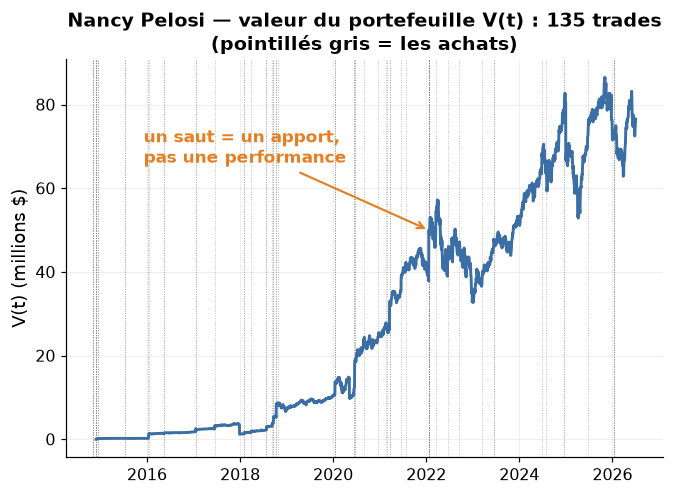
\includegraphics[width=0.86\linewidth]{fig_05b_pelosi_valeur.png}\\[1mm]
      {\scriptsize\color{black!60} exemple réel : $V(t)$ d'un membre — la brique
       de la stratégie S3 ; brancher le \textbf{patrimoine d'entrée (H)} comme
       capital initial est la suite prévue}
    \end{column}
  \end{columns}
\end{frame}

% ── H15 · Les résultats ── (MANIFEST : C-a 78,7 · C-b 85,0 · O4 83,7 · C-d/C-e 0 ; fig_v1_coherence)
\begin{frame}{Résultat — les portefeuilles se recoupent, et les trous s'expliquent}
  \centering
  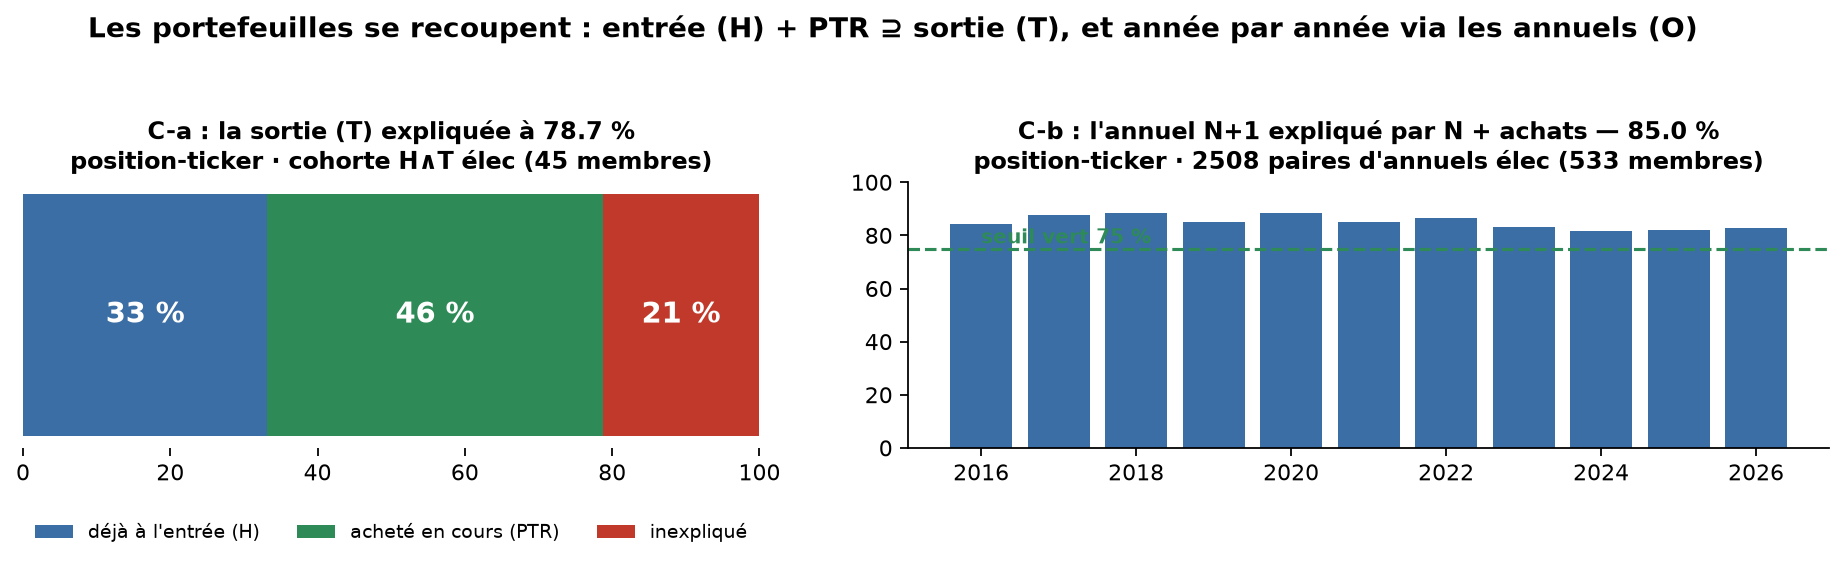
\includegraphics[width=0.88\textwidth]{fig_v1_coherence.png}\\[1.5mm]
  \begin{columns}[T]
    \begin{column}{0.52\textwidth}
      {\footnotesize
      · \badge{okgreen}{C-a = 78,7 \%} des positions de sortie expliquées
        (45 membres entrés ET sortis, H∧T électroniques)\\[1mm]
      · \badge{okgreen}{C-b = 85,0 \%} l'annuel N+1 expliqué par l'annuel N + achats
        (2\,508 paires, 533 membres)\\[1mm]
      · \badge{okgreen}{O4 = 83,7 \%} des \textbf{actions} des annuels retrouvées
        en PTR — fonds et ETF : \textbf{exemptés par la loi}, pas ratés}
    \end{column}
    \begin{column}{0.46\textwidth}
      {\scriptsize\color{black!70}
      \textbf{et le 21 \% inexpliqué ?} réglé \textbf{un par un} — slide
      suivante. Une certitude d'abord : \textbf{0 blind trust}
      (C-d = C-e = 0) — le trust, lui, fait \emph{disparaître} :
      Dean Phillips entre avec \textbf{284} positions, sort avec \textbf{1}
      ligne opaque « \emph{Qualified Blind Trust [EQ]} », sans ticker.}
    \end{column}
  \end{columns}
\end{frame}

% ── H15b · Les 292 trous un par un ── (§16 ; C-a-ocr 78,8 · C-a2 84,2 · C-a2t 87,8 · C-f 3,3)
\begin{frame}{Les 21 \% inexpliqués, réglés un par un — il en reste 3,3 \%}
  \centering
  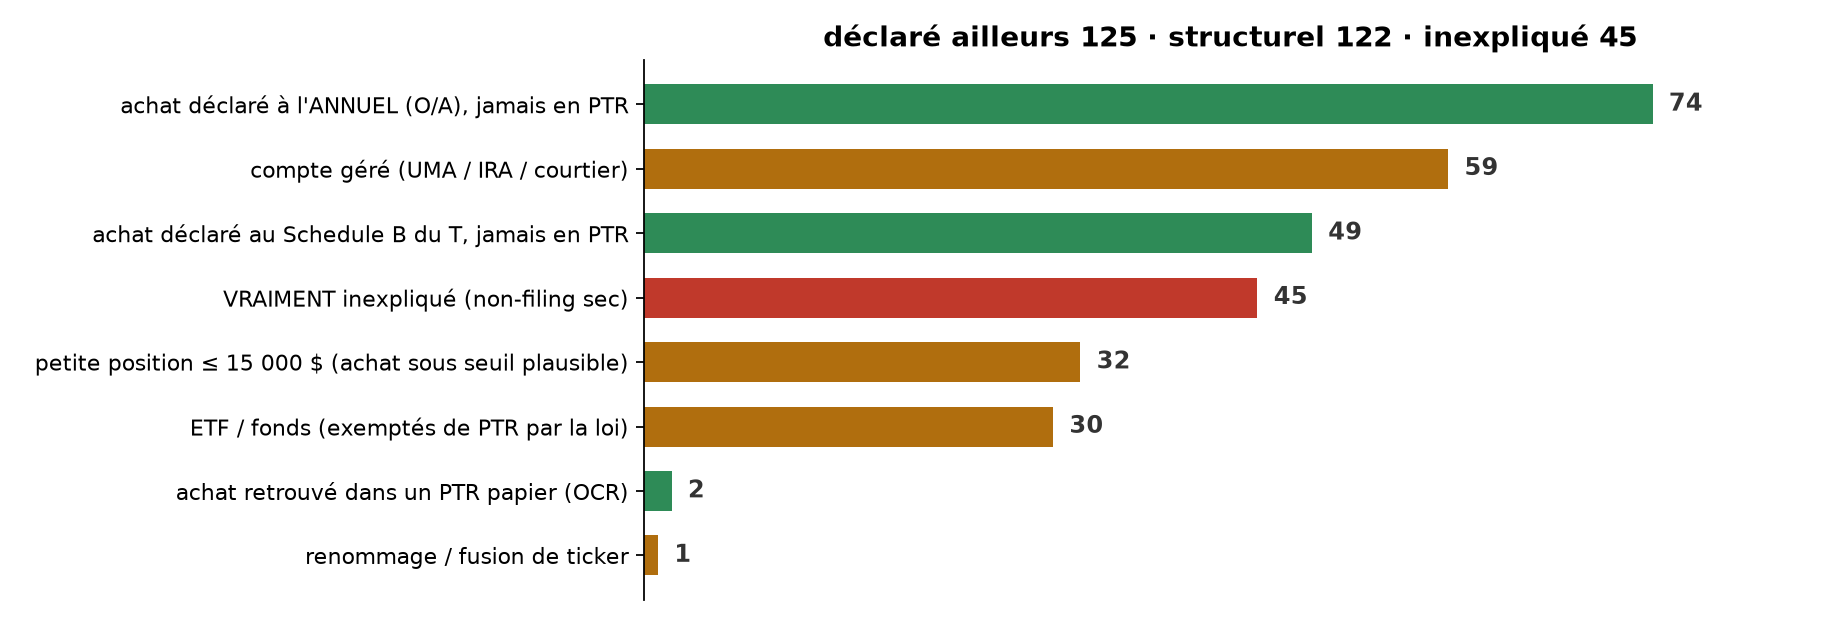
\includegraphics[width=0.82\textwidth]{fig_house_trous.png}\\[1.5mm]
  \begin{columns}[T]
    \begin{column}{0.56\textwidth}
      {\footnotesize en comptant \textbf{toutes} les déclarations d'achat (PTR élec
      \textbf{78,7 \%} → + PTR papier \textbf{78,8 \%} → + annuels O/A
      \textbf{84,2 \%} → + Schedule B du T \textbf{87,8 \%}) : 125 « trous » sont
      des trades \textbf{déclarés par l'élu lui-même}… hors PTR — du
      \textbf{non-filing documenté} (délai STOCK Act non respecté), pas un trou
      de collecte. Mitchell : 32/43 · Manning : 25/28.}
    \end{column}
    \begin{column}{0.42\textwidth}
      \badge{okgreen}{C-f = 3,3 \% vraiment inexpliqué}\\[1.5mm]
      {\scriptsize\color{black!60} 45 positions chez 14 membres ; le reste est
       structurel (comptes gérés, ETF exemptés, sous le seuil des 1\,000 \$) —
       table nominative : \co{annexe\_coherence\_trous\_v1.csv}}
    \end{column}
  \end{columns}
\end{frame}

% ── H15c · B3 : le patrimoine papier OCRisé ── (§17 ; F1 526 · F4 78,3 · F5 87,1 · F6 54)
\begin{frame}{B3 — le patrimoine papier, lu à son tour : la conclusion tient}
  \centering
  {\footnotesize 556 photos scannées OCRisées — 12 H + 100 T + 444 annuels $\leq$ 12 pages,
   $\approx$ 50 \$ — dont 526 avec contenu → \textbf{15\,489 holdings papier},
   cache versionné \co{reference/ocr\_cache\_fd\_v1/}}\\[2mm]
  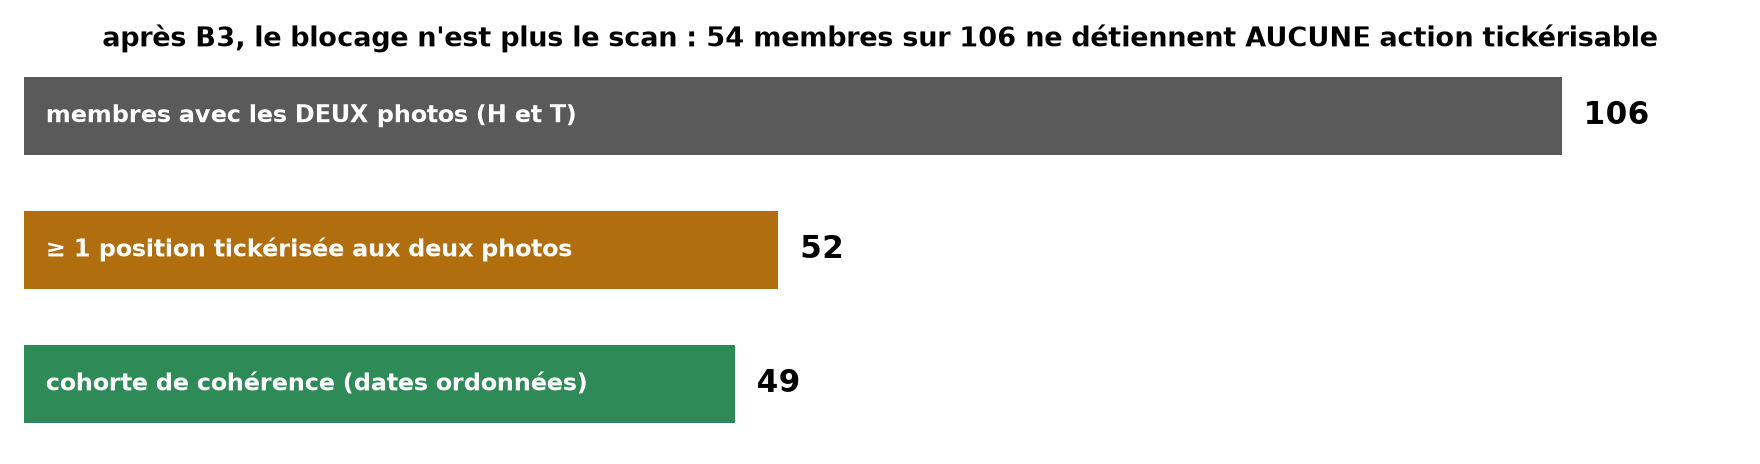
\includegraphics[width=0.79\textwidth]{fig_house_entonnoir_b3.png}\\[1mm]
  \begin{columns}[T]
    \begin{column}{0.55\textwidth}
      {\footnotesize la cohorte passe de 45 à \textbf{49 membres} (+ Dold, Guinta,
      Lawrence, Trott) et les taux \textbf{tiennent} : \badge{okgreen}{78,3 \% (achats PTR)}
      \badge{okgreen}{87,1 \% toutes déclarations}}
    \end{column}
    \begin{column}{0.43\textwidth}
      {\scriptsize\color{black!60} restent hors d'atteinte d'un suivi par ticker :
       54 membres à patrimoine fonds/comptes/immobilier · les 276 annuels-monstres
       (annexes de courtier, $\approx$ 267 \$) : décision séparée}
    \end{column}
  \end{columns}
\end{frame}

% ── H16 · Le tableau de bord ── (MANIFEST.json : 57 validations, 0 rouge ; fig_house_dashboard)
\begin{frame}{Le tableau de bord — 57 validations, 0 rouge}
  \centering
  
\includegraphics[width=0.585\textwidth]{fig_house_dashboard.png}
\end{frame}

\section{Verdict}

% ── H17 · Conclusion ── (comptes MANIFEST : 161 076 signal · 198 615 holdings · 24 078 PDF)
\begin{frame}{Ce que ce deck prouve — et la suite}
  \centering
  \tuile{helec}{161\,076}{transactions PTR\\= le signal, couvert à 100\,\%}\hfill
  \tuile{dataC}{198\,615}{holdings Schedule A\\(photos de patrimoine)}\hfill
  \tuile{grisC}{24\,078}{PDF archivés\\+ index irremplaçables}\hfill
  \tuile{okgreen}{57 / 0}{validations / rouge\\tout re-jouable}\\[5mm]
  {\footnotesize
  \badge{helec}{1. source exhaustive et archivée — le site détruit (5 U.S.C. §13107), pas nous}\\[1.5mm]
  \badge{helec}{2. tri lisible/scanné mesuré (0 désaccord) — l'OCR au strict nécessaire}\\[1.5mm]
  \badge{helec}{3. chaque portefeuille se recoupe — 87,8 \% toutes déclarations, 3,3 \% d'inexpliqué}}\\[4mm]
  {\scriptsize\color{black!60} suites naturelles : le Sénat sur le même modèle ·
   appariement par NOM d'actif (les 54 membres sans ticker) et les 276 annuels-monstres ·
   brancher le patrimoine d'entrée (H) dans le moteur de stratégie S3}
\end{frame}



\end{document}
